\documentclass{beamer}
\usepackage[english]{babel}      
\usepackage[T1]{fontenc}      
\usepackage[latin1]{inputenc} 
\usepackage{geometry}        
\usepackage{alltt}        
\usepackage{color}        

\usepackage{amsmath,amsfonts,amssymb} 
\usepackage{amsthm}                  
\usepackage{graphicx}               
\usepackage{subfig}                
% \usepackage{hyperref}                
                                 
\usepackage{listings}           
\usepackage{minted}           


\usetheme{Warsaw}

\newcommand{\E}[1]{\times 10^{#1}}
\newcommand{\pdiff}[3][\null]{\frac{\partial^{#1}{#2}}{\partial{#3}^{#1}}}
\newcommand{\vect}[1]{\mbox{\boldmath{$#1$}}}
\newcommand{\Lapl}{\nabla^2}
\newcommand{\Grad}{\mbox{\boldmath{$\nabla$}}}
\newcommand{\vdot}{\mathop{\mbox{\boldmath{$\cdot$}}}}
\newcommand{\Div}{\Grad\vdot}
\newcommand{\units}[1]{\,\mathrm{#1}}
\newcommand{\boxmath}[1]{\begin{displaymath}\fbox{$\displaystyle#1$}\end{displaymath}}


\graphicspath{{./}{Figures/}}


\theoremstyle{plain}
\newtheorem{observasjon}{Observasjon}

\theoremstyle{definition}
\newtheorem{definisjon}{Definisjon}


\title{Geomodeller revisited}
\author{Brief introduction to GeoModeler}
\institute{Kjetil A. Johannessen}
\date{January 14, 2016}

\begin{document}

%%%%%%%%%%%%%%%%%%%%%%%%%%%%%%%%%%%%%%%%%%%%%%%%%%%%%%%%%%%%%%%%%%%%%%%%%%%%%%%%%%%%%%%%%%%%%%%%%%%%%%%%%%%%%%%%%
\begin{frame}
\titlepage
\end{frame}
%%%%%%%%%%%%%%%%%%%%%%%%%%%%%%%%%%%%%%%%%%%%%%%%%%%%%%%%%%%%%%%%%%%%%%%%%%%%%%%%%%%%%%%%%%%%%%%%%%%%%%%%%%%%%%%%%
%%%%%%%%%%%%%%%%%%%%%%%%%%%%%%%%%%%%%%%%%%%%%%%%%%%%%%%%%%%%%%%%%%%%%%%%%%%%%%%%%%%%%%%%%%%%%%%%%%%%%%%%%%%%%%%%%
%\section{Introduction}
\begin{frame}
\frametitle{Why fix the geomodeller}
\textbf{Why fix the geomodeller}

GoTools is lacking in several places
\begin{itemize}
    \item Incomplete
    \item Unstable
    \item Inconsistent
    \item Unresponsive
\end{itemize}
Technical difficulties by writing C in python
\end{frame}

%%%%%%%%%%%%%%%%%%%%%%%%%%%%%%%%%%%%%%%%%%%%%%%%%%%%%%%%%%%%%%%%%%%%%%%%%%%%%%%%%%%%%%%%%%%%%%%%%%%%%%%%%%%%%%%%%

\begin{frame}
\frametitle{Other IGA and modelling libraries}
\textbf{Other IGA and modelling libraries}

\begin{itemize}
    \item GeoPDE - University of Pavia
    \item IGAkit - King Abdullah University of Science and Technology
\end{itemize}
All have very weak modelling capabilities
\end{frame}

%%%%%%%%%%%%%%%%%%%%%%%%%%%%%%%%%%%%%%%%%%%%%%%%%%%%%%%%%%%%%%%%%%%%%%%%%%%%%%%%%%%%%%%%%%%%%%%%%%%%%%%%%%%%%%%%%

\begin{frame}
\frametitle{Other CAD tools}
\textbf{Other CAD tools}

\begin{itemize}
    \item Rhinoceros 3D
    \item SolidWorks 
\end{itemize}
are proprietaire software.

\pause
\vspace{1cm}
Open source alternatives include:
\begin{itemize}
    \item FreeCAD   - no splines, lots of crashbugs
    \item Blender   - for artists
    \item openNURBS - C++ library, used by Rhino 3D
\end{itemize}
\pause
but still no volumetric modelling capabilities.
\end{frame}

%%%%%%%%%%%%%%%%%%%%%%%%%%%%%%%%%%%%%%%%%%%%%%%%%%%%%%%%%%%%%%%%%%%%%%%%%%%%%%%%%%%%%%%%%%%%%%%%%%%%%%%%%%%%%%%%%

\begin{frame}[fragile]
\frametitle{Closest design cousin:}
\textbf{GMSH:}
\begin{columns}
    \begin{column}{.50\linewidth}
        \begin{listing}[H]
            \tiny
            \begin{minted}{c++}
cm = 1e-02;
e1 = 4.5 * cm; e2 = 6 * cm / 2; e3 =  5 * cm / 2;
// ...

Point(1) = {-e1-e2, 0    , 0, Lc1};
Point(2) = {-e1-e2, h1   , 0, Lc1};
// ...
Point(24)= { 0, h1+h3+h4+R2, 0, Lc2};
Point(25)= { 0, h1+h3-R2,    0, Lc2};

Line(1)  = {1 , 17};
Line(2)  = {17, 16};

Circle(3) = {14,15,16};

Line(4)  = {14,13};
// ...
Circle(8) = {8,9,10};
Line(9)  = {8,7};
// ...
Line(20) = {21,22};

Line Loop(21) = {17,-15,18,19,-20,16};
Plane Surface(22) = {21};
            \end{minted}
        \end{listing}
    \end{column}
    \begin{column}{.45\linewidth}
        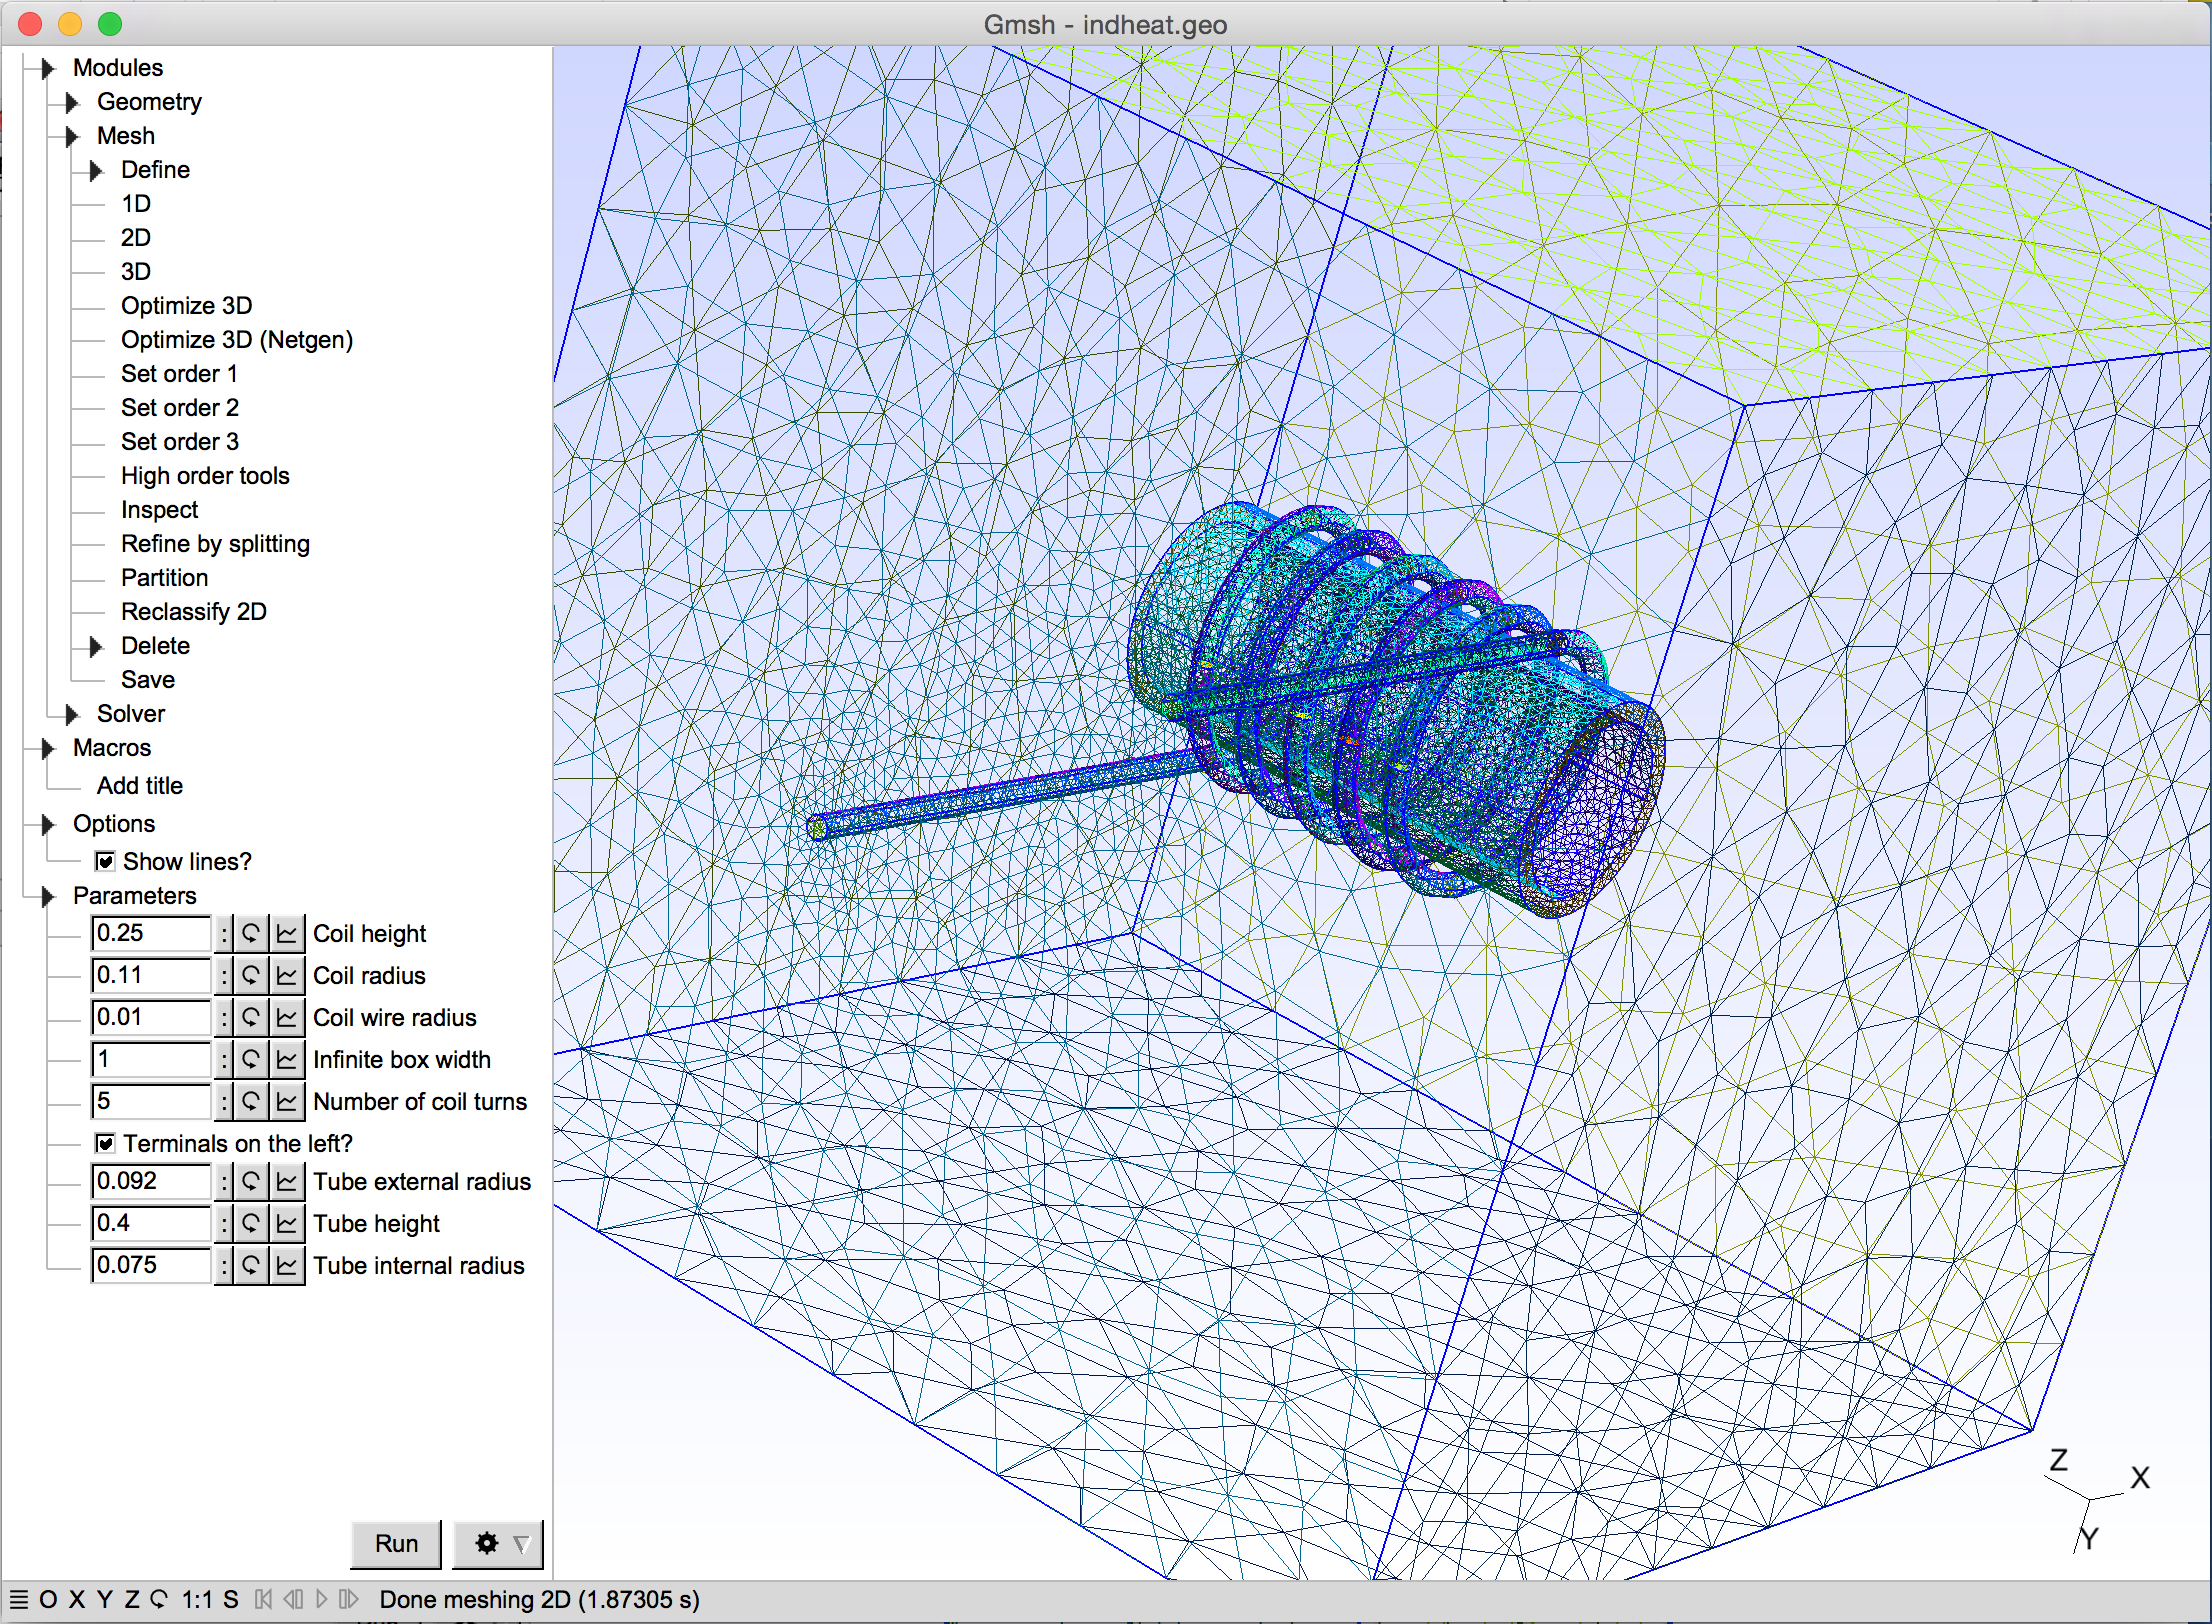
\includegraphics[width=\linewidth]{gmsh}
    \end{column}
\end{columns}


\end{frame}

%%%%%%%%%%%%%%%%%%%%%%%%%%%%%%%%%%%%%%%%%%%%%%%%%%%%%%%%%%%%%%%%%%%%%%%%%%%%%%%%%%%%%%%%%%%%%%%%%%%%%%%%%%%%%%%%%

\begin{frame}[fragile]
\frametitle{Closest design cousin:}
\textbf{OpenSCAD:}
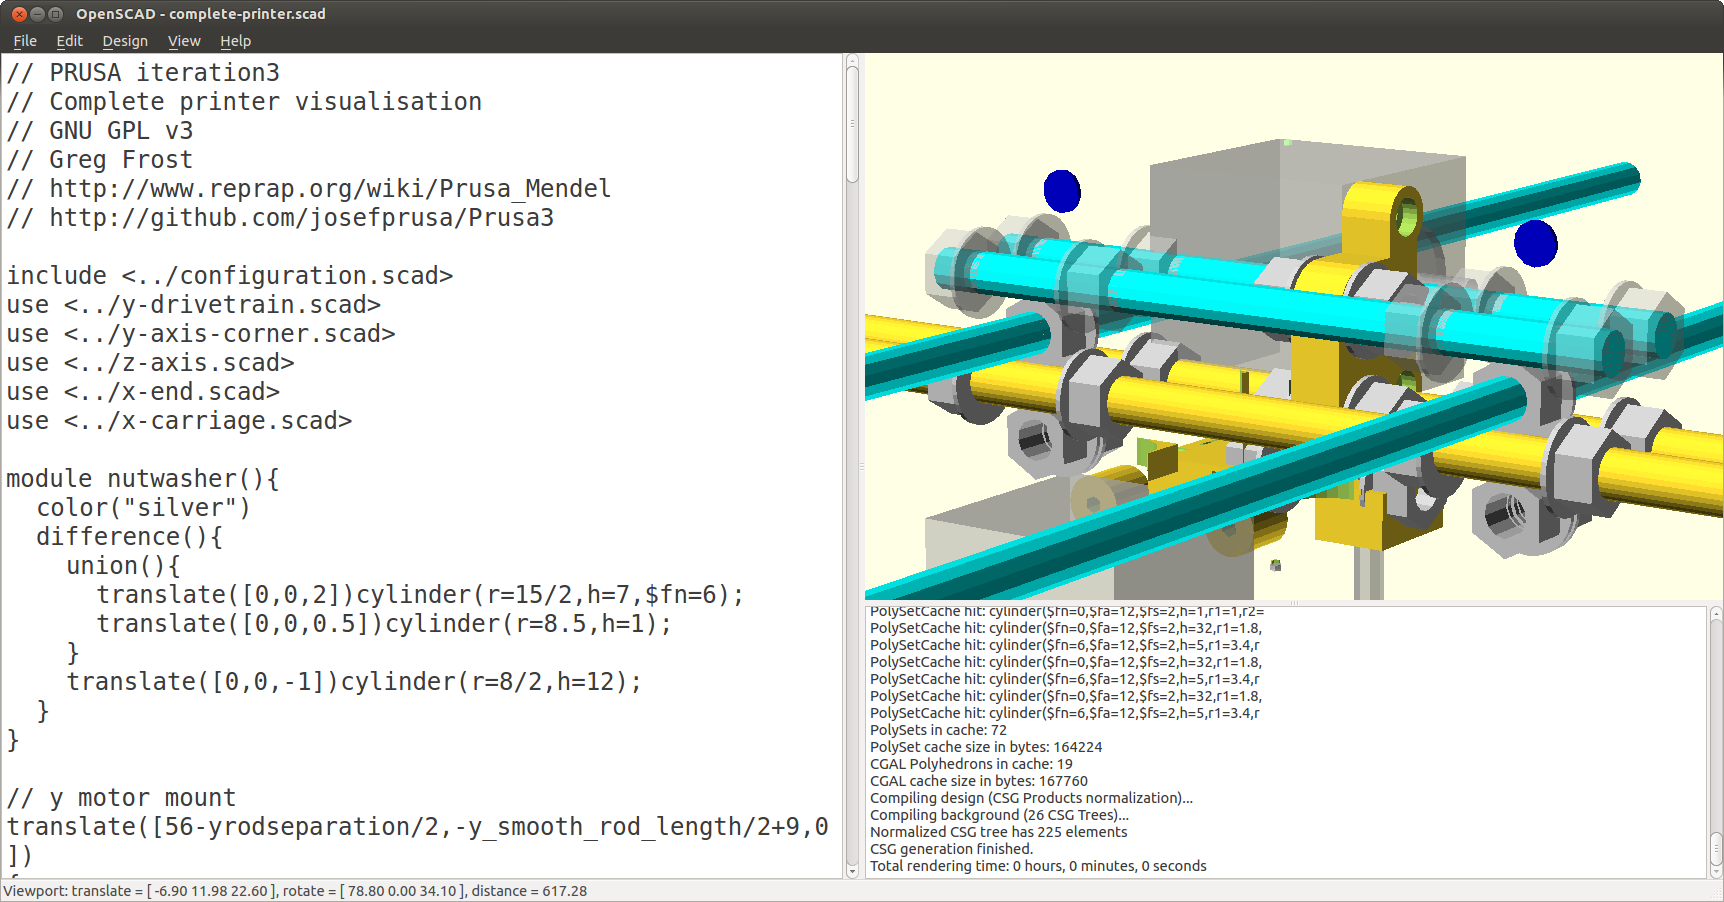
\includegraphics[width=0.9\linewidth]{openscad}

\end{frame}

%%%%%%%%%%%%%%%%%%%%%%%%%%%%%%%%%%%%%%%%%%%%%%%%%%%%%%%%%%%%%%%%%%%%%%%%%%%%%%%%%%%%%%%%%%%%%%%%%%%%%%%%%%%%%%%%%

\begin{frame}
\frametitle{We need}
\textbf{We need}

\begin{itemize}
    \item Analysis ready
    \begin{itemize}
        \item watertight
        \item non-overlapping
        \item conforming
    \end{itemize}
    \item Volumetric (trivariate) modelling support
    \item Scriptable
    \item Full discretization control
\end{itemize}
\pause
\vspace{1cm}
\textit{Easy to learn, hard to master}

\end{frame}

%%%%%%%%%%%%%%%%%%%%%%%%%%%%%%%%%%%%%%%%%%%%%%%%%%%%%%%%%%%%%%%%%%%%%%%%%%%%%%%%%%%%%%%%%%%%%%%%%%%%%%%%%%%%%%%%%

\begin{frame}
\frametitle{Basics}
\textbf{Basics}

Based on python 
\begin{itemize}
    \item Fairly easy scripting language
    \item Full power of numpy (C fast linear algebra)
\end{itemize}
\pause
\vspace{1cm}
You make geometries by
\begin{itemize}
    \item Creating curves from points
    \item Creating surfaces from curves
    \item Creating volumes from surfaces
\end{itemize}
...roughly speaking

\end{frame}

%%%%%%%%%%%%%%%%%%%%%%%%%%%%%%%%%%%%%%%%%%%%%%%%%%%%%%%%%%%%%%%%%%%%%%%%%%%%%%%%%%%%%%%%%%%%%%%%%%%%%%%%%%%%%%%%%

\begin{frame}[fragile]
\frametitle{Examples:}
\textbf{Examples:}
\begin{columns}
    \begin{column}{.50\linewidth}
        \begin{listing}[H]
            \tiny
            \begin{minted}{python}
from math import *
import CurveFactory                                                            


                                                                               
myLine = CurveFactory.line([0,0],  [-3,2])                                   
myArc  = CurveFactory.circle_segment(pi/4)                                     










# write results to file                                                        
f = open('tutorial.g2', 'w')                                                   
myLine.write_g2(f)
myArc.write_g2(f)
            \end{minted}
        \end{listing}
    \end{column}
    \begin{column}{.45\linewidth}
        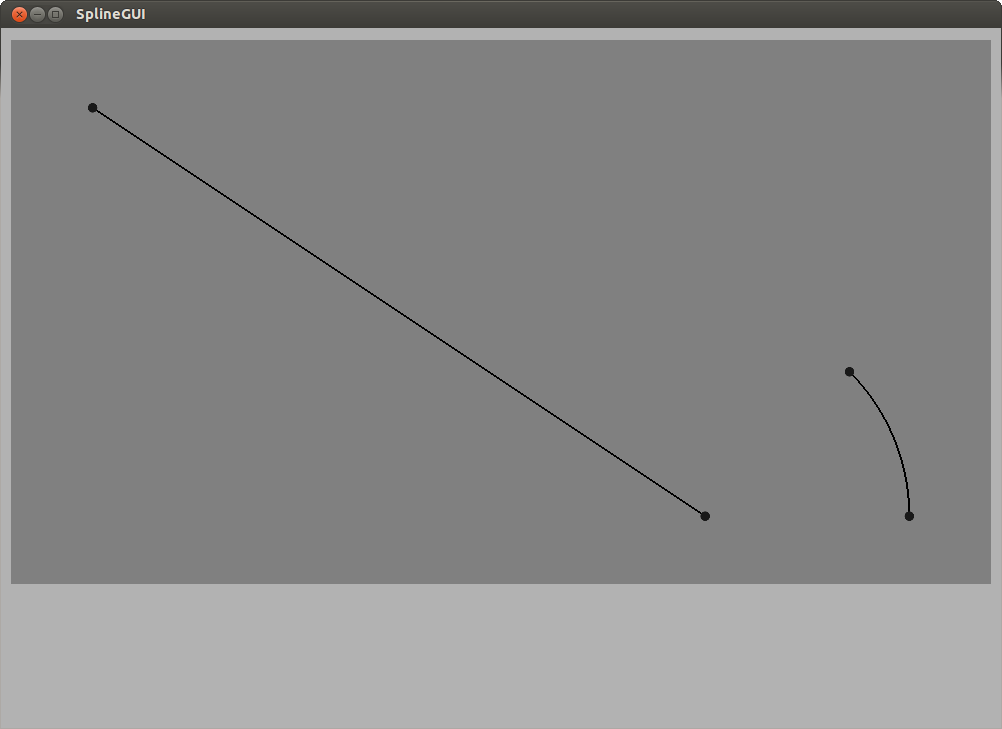
\includegraphics[width=\linewidth]{tutorial1}
    \end{column}
\end{columns}

\end{frame}

%%%%%%%%%%%%%%%%%%%%%%%%%%%%%%%%%%%%%%%%%%%%%%%%%%%%%%%%%%%%%%%%%%%%%%%%%%%%%%%%%%%%%%%%%%%%%%%%%%%%%%%%%%%%%%%%%

\begin{frame}[fragile]
\frametitle{Examples:}
\textbf{Examples:}
\begin{columns}
    \begin{column}{.50\linewidth}
        \begin{listing}[H]
            \tiny
            \begin{minted}{python}
from math import *
import CurveFactory                                                            
import SurfaceFactory                                                            

                                                                               
myLine = CurveFactory.line([0,0],  [-3,2])                                   
myArc  = CurveFactory.circle_segment(pi/4)                                     

mySurface = SurfaceFactory.edge_curves([myLine, myArc])








                                                                               
# write results to file                                                        
f = open('tutorial.g2', 'w')                                                   
mySurface.write(f)

            \end{minted}
        \end{listing}
    \end{column}
    \begin{column}{.45\linewidth}
        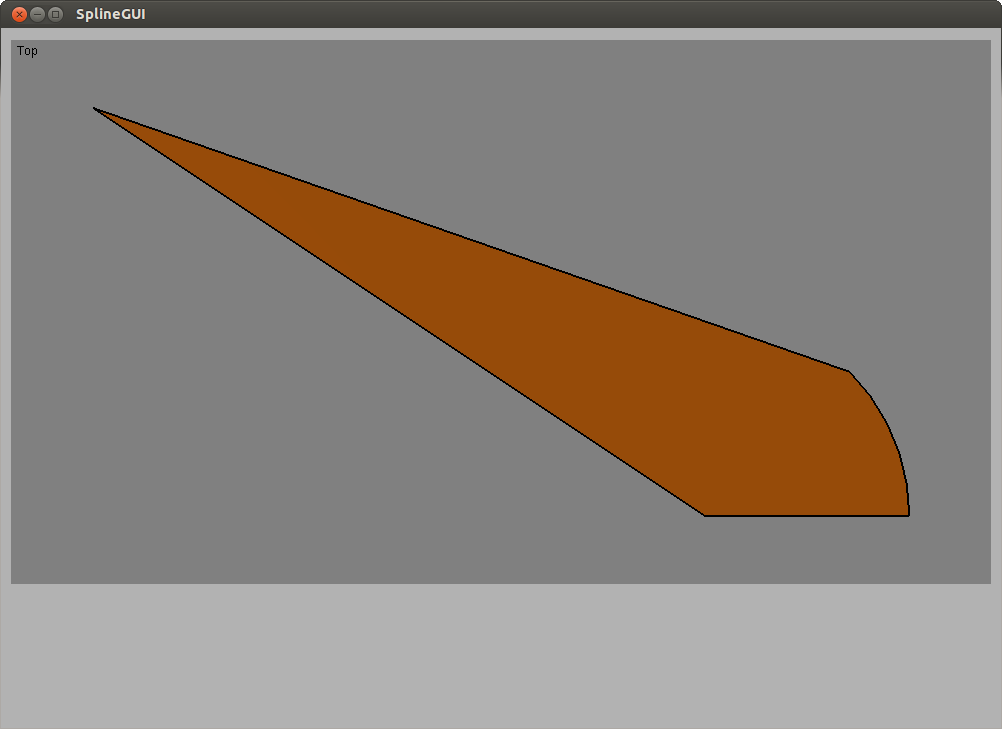
\includegraphics[width=\linewidth]{tutorial2}
    \end{column}
\end{columns}

\end{frame}

%%%%%%%%%%%%%%%%%%%%%%%%%%%%%%%%%%%%%%%%%%%%%%%%%%%%%%%%%%%%%%%%%%%%%%%%%%%%%%%%%%%%%%%%%%%%%%%%%%%%%%%%%%%%%%%%%

\begin{frame}[fragile]
\frametitle{Examples:}
\textbf{Examples:}
\begin{columns}
    \begin{column}{.50\linewidth}
        \begin{listing}[H]
            \tiny
            \begin{minted}{python}
from math import *
import CurveFactory                                                            
import SurfaceFactory                                                            

                                                                               
myLine = CurveFactory.line([0,0],  [-3,2])                                   
myArc  = CurveFactory.circle_segment(pi/4)                                     

mySurface = SurfaceFactory.edge_curves([myLine, myArc])
mySurface.refine(5)







                                                                               
# write results to file                                                        
f = open('tutorial.g2', 'w')                                                   
mySurface.write(f)

            \end{minted}
        \end{listing}
    \end{column}
    \begin{column}{.45\linewidth}
        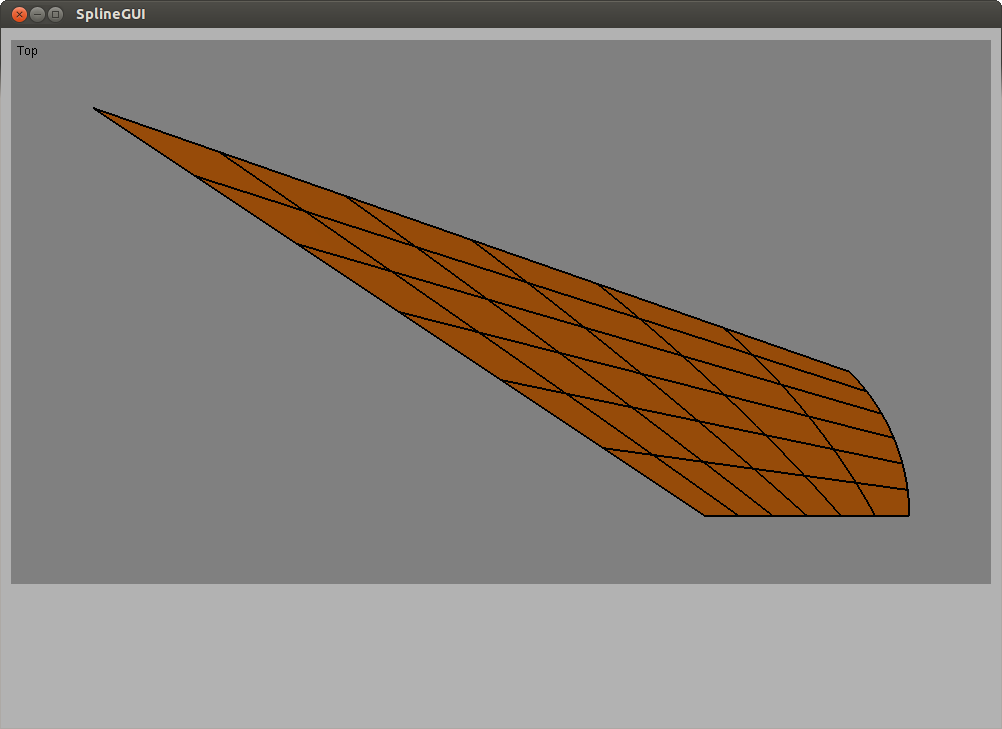
\includegraphics[width=\linewidth]{tutorial3}
    \end{column}
\end{columns}

\end{frame}

%%%%%%%%%%%%%%%%%%%%%%%%%%%%%%%%%%%%%%%%%%%%%%%%%%%%%%%%%%%%%%%%%%%%%%%%%%%%%%%%%%%%%%%%%%%%%%%%%%%%%%%%%%%%%%%%%

\begin{frame}[fragile]
\frametitle{Examples:}
\textbf{Examples:}
\begin{columns}
    \begin{column}{.50\linewidth}
        \begin{listing}[H]
            \tiny
            \begin{minted}{python}
from math import *
import CurveFactory                                                            
import SurfaceFactory                                                            
import VolumeFactory                                                            
                                                                               
myLine = CurveFactory.line([0,0],  [-3,2])                                   
myArc  = CurveFactory.circle_segment(pi/4)                                     

mySurface = SurfaceFactory.edge_curves([myLine, myArc])
mySurface.refine(5)

mySurface.translate((2,0,0))    # move 2 in x-direction
mySurface = mySurface + (2,0,0) # move 2 in x-direction
mySurface += (1,0,0)            # move 1 in x-direction
mySurface.rotate(pi/2, (1,0,0)) # rotate into xz-plane

myVolume = VolumeFactory.revolve(mySurface)
                                                                               
# write results to file                                                        
f = open('tutorial.g2', 'w')                                                   
myVolume.write(f)

            \end{minted}
        \end{listing}
    \end{column}
    \begin{column}{.45\linewidth}
        \only<1>{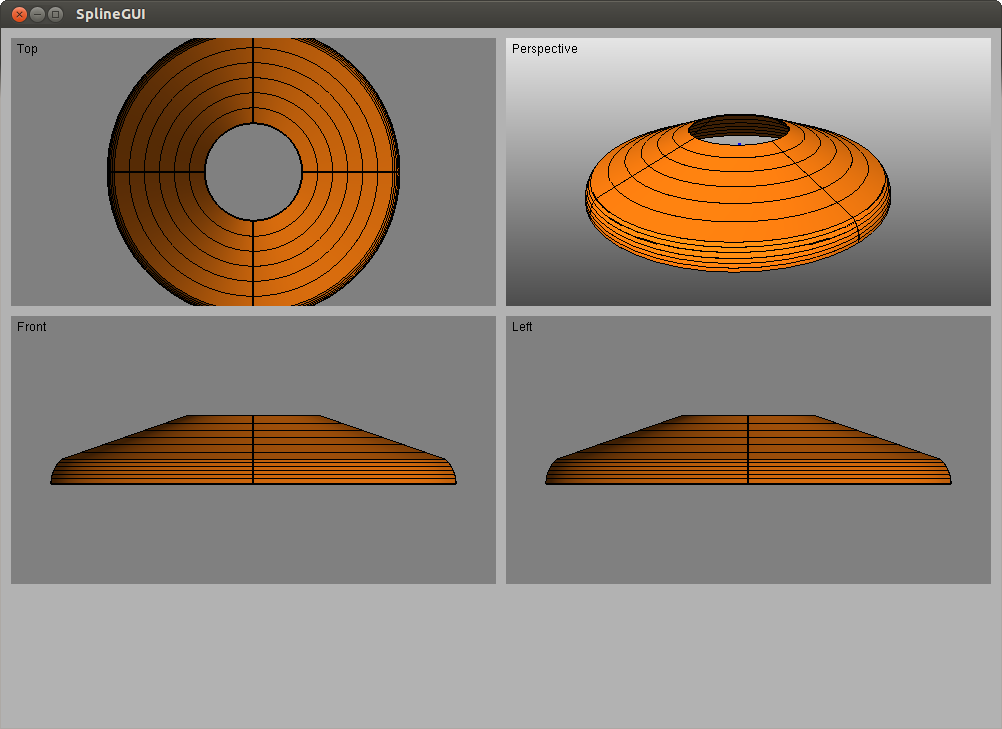
\includegraphics[width=\linewidth]{tutorial4}}
        \only<2>{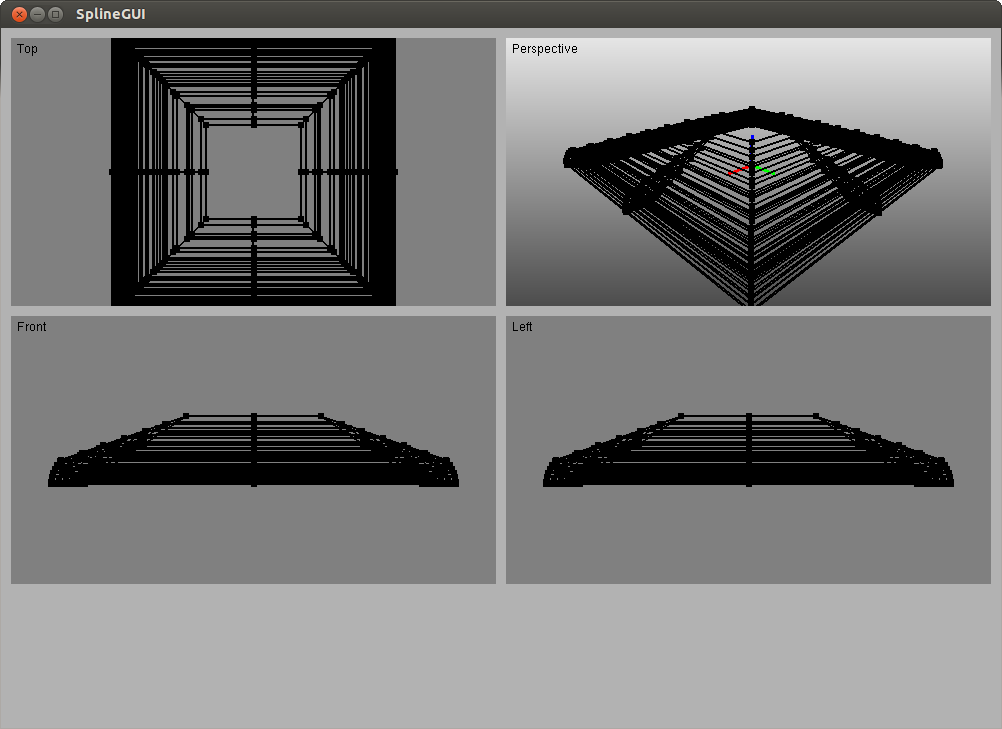
\includegraphics[width=\linewidth]{tutorial5}}
    \end{column}
\end{columns}

\end{frame}

%%%%%%%%%%%%%%%%%%%%%%%%%%%%%%%%%%%%%%%%%%%%%%%%%%%%%%%%%%%%%%%%%%%%%%%%%%%%%%%%%%%%%%%%%%%%%%%%%%%%%%%%%%%%%%%%%

\begin{frame}[fragile]
\frametitle{Examples:}
\textbf{Examples:}
\begin{columns}
    \begin{column}{.50\linewidth}
        \begin{listing}[H]
            \tiny
            \begin{minted}{python}
import CurveFactory   as cf
import SurfaceFactory as sf
from math import pi

x  = cf.line([-.5, 0], [.5, 0]) # just to show the origin
y  = cf.line([0, -.5], [0, .5]) # just to show the origin

c1 = cf.circle_segment(pi/2)
c2 = cf.line([0,1], [-4,1])
c1.append(c2)











f = open('ntnu.g2', 'w')
c1.write_g2(f)

x.write_g2(f)
y.write_g2(f)
            \end{minted}
        \end{listing}
    \end{column}
    \begin{column}{.45\linewidth}
        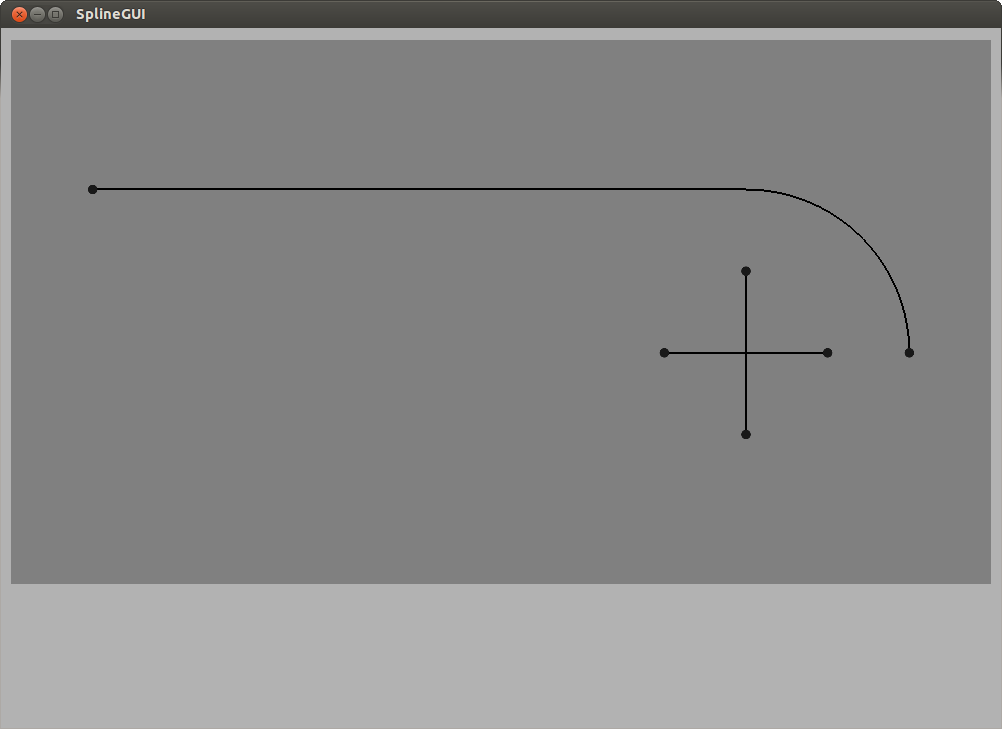
\includegraphics[width=\linewidth]{ntnu1}
    \end{column}
\end{columns}

\end{frame}

%%%%%%%%%%%%%%%%%%%%%%%%%%%%%%%%%%%%%%%%%%%%%%%%%%%%%%%%%%%%%%%%%%%%%%%%%%%%%%%%%%%%%%%%%%%%%%%%%%%%%%%%%%%%%%%%%

\begin{frame}[fragile]
\frametitle{Examples:}
\textbf{Examples:}
\begin{columns}
    \begin{column}{.50\linewidth}
        \begin{listing}[H]
            \tiny
            \begin{minted}{python}
import CurveFactory   as cf
import SurfaceFactory as sf
from math import pi

x  = cf.line([-.5, 0], [.5, 0]) # just to show the origin
y  = cf.line([0, -.5], [0, .5]) # just to show the origin

c1 = cf.circle_segment(pi/2)
c2 = cf.line([0,1], [-4,1])
c1.append(c2)
c1 += (2, 2)
c2 = c1.clone().rotate(pi/2)
c1.append(c2)








f = open('ntnu.g2', 'w')
c1.write_g2(f)

x.write_g2(f)
y.write_g2(f)
            \end{minted}
        \end{listing}
    \end{column}
    \begin{column}{.45\linewidth}
        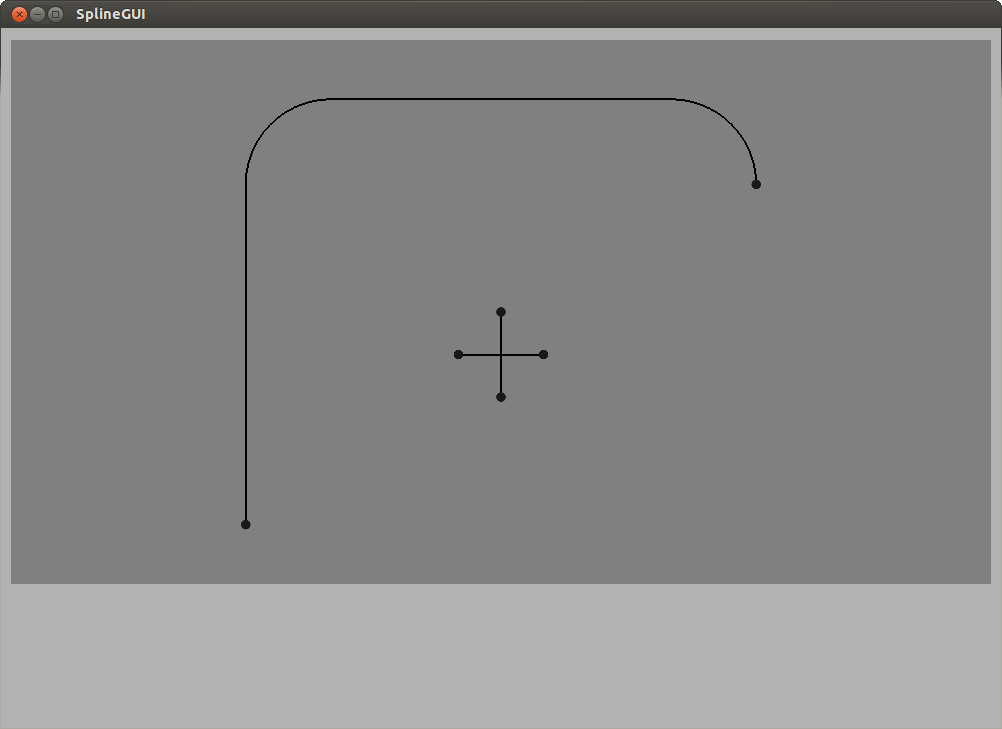
\includegraphics[width=\linewidth]{ntnu2}
    \end{column}
\end{columns}

\end{frame}

%%%%%%%%%%%%%%%%%%%%%%%%%%%%%%%%%%%%%%%%%%%%%%%%%%%%%%%%%%%%%%%%%%%%%%%%%%%%%%%%%%%%%%%%%%%%%%%%%%%%%%%%%%%%%%%%%

\begin{frame}[fragile]
\frametitle{Examples:}
\textbf{Examples:}
\begin{columns}
    \begin{column}{.50\linewidth}
        \begin{listing}[H]
            \tiny
            \begin{minted}{python}
import CurveFactory   as cf
import SurfaceFactory as sf
from math import pi

x  = cf.line([-.5, 0], [.5, 0]) # just to show the origin
y  = cf.line([0, -.5], [0, .5]) # just to show the origin

c1 = cf.circle_segment(pi/2)
c2 = cf.line([0,1], [-4,1])
c1.append(c2)
c1 += (2, 2)
c2 = c1.clone().rotate(pi/2)
c1.append(c2)
c2 = c1.clone().rotate(pi)
c1.append(c2)






f = open('ntnu.g2', 'w')
c1.write_g2(f)

x.write_g2(f)
y.write_g2(f)
            \end{minted}
        \end{listing}
    \end{column}
    \begin{column}{.45\linewidth}
        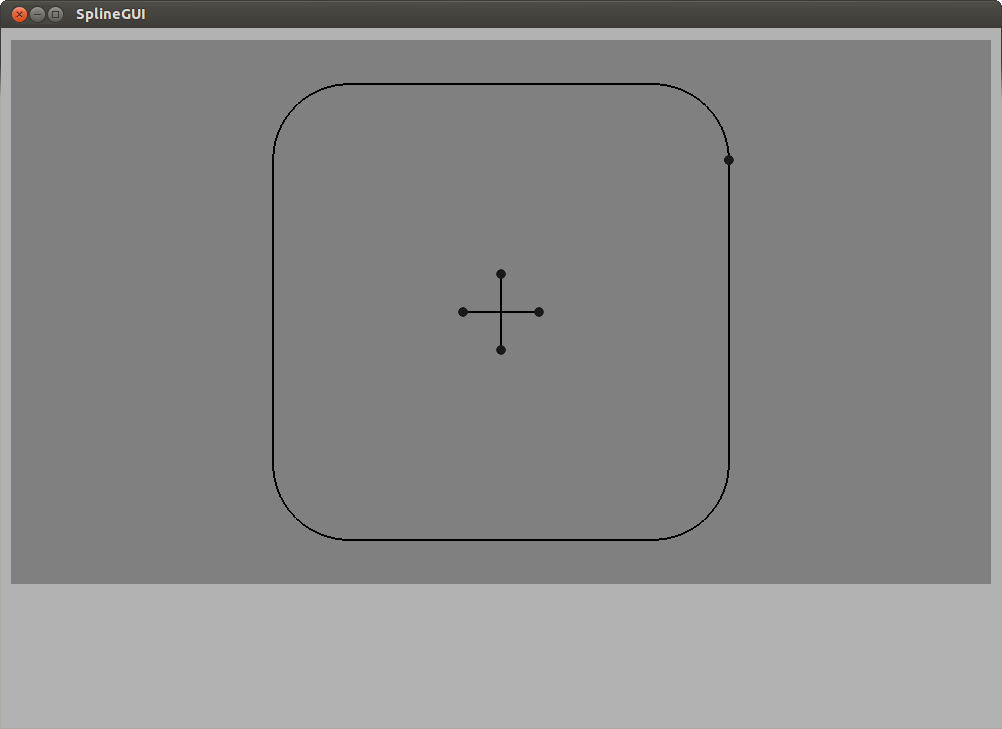
\includegraphics[width=\linewidth]{ntnu3}
    \end{column}
\end{columns}

\end{frame}

%%%%%%%%%%%%%%%%%%%%%%%%%%%%%%%%%%%%%%%%%%%%%%%%%%%%%%%%%%%%%%%%%%%%%%%%%%%%%%%%%%%%%%%%%%%%%%%%%%%%%%%%%%%%%%%%%

\begin{frame}[fragile]
\frametitle{Examples:}
\textbf{Examples:}
\begin{columns}
    \begin{column}{.50\linewidth}
        \begin{listing}[H]
            \tiny
            \begin{minted}{python}
import CurveFactory   as cf
import SurfaceFactory as sf
from math import pi

x  = cf.line([-.5, 0], [.5, 0]) # just to show the origin
y  = cf.line([0, -.5], [0, .5]) # just to show the origin

c1 = cf.circle_segment(pi/2)
c2 = cf.line([0,1], [-4,1])
c1.append(c2)
c1 += (2, 2)
c2 = c1.clone().rotate(pi/2)
c1.append(c2)
c2 = c1.clone().rotate(pi)
c1.append(c2)

s1 = sf.thicken(c1, 1)




f = open('ntnu.g2', 'w')
s1.write_g2(f)

x.write_g2(f)
y.write_g2(f)
            \end{minted}
        \end{listing}
    \end{column}
    \begin{column}{.45\linewidth}
        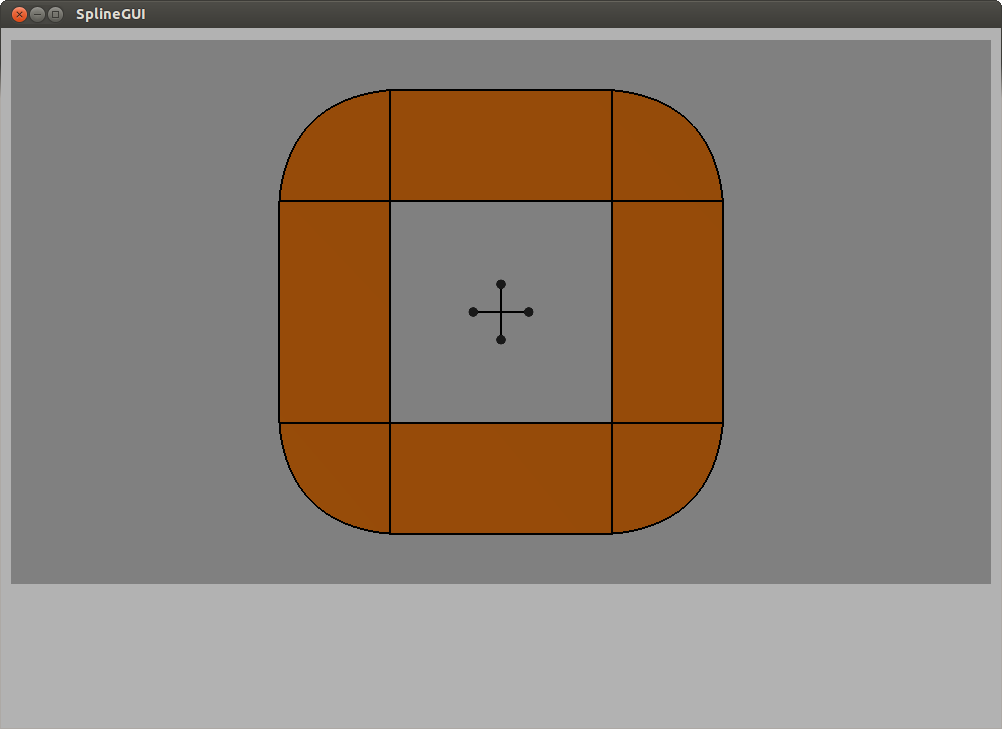
\includegraphics[width=\linewidth]{ntnu4}
    \end{column}
\end{columns}

\end{frame}

%%%%%%%%%%%%%%%%%%%%%%%%%%%%%%%%%%%%%%%%%%%%%%%%%%%%%%%%%%%%%%%%%%%%%%%%%%%%%%%%%%%%%%%%%%%%%%%%%%%%%%%%%%%%%%%%%

\begin{frame}[fragile]
\frametitle{Examples:}
\textbf{Examples:}
\begin{columns}
    \begin{column}{.50\linewidth}
        \begin{listing}[H]
            \tiny
            \begin{minted}{python}
import CurveFactory   as cf
import SurfaceFactory as sf
from math import pi

x  = cf.line([-.5, 0], [.5, 0]) # just to show the origin
y  = cf.line([0, -.5], [0, .5]) # just to show the origin

c1 = cf.circle_segment(pi/2)
c2 = cf.line([0,1], [-4,1])
c1.append(c2)
c1 += (2, 2)
c2 = c1.clone().rotate(pi/2)
c1.append(c2)
c2 = c1.clone().rotate(pi)
c1.append(c2)

s1 = sf.thicken(c1, 1)
s2 = sf.disc(1.5)
s1.refine(2)
s2.refine(3)

f = open('ntnu.g2', 'w')
s1.write_g2(f)

# x.write_g2(f)
# y.write_g2(f)
            \end{minted}
        \end{listing}
    \end{column}
    \begin{column}{.45\linewidth}
        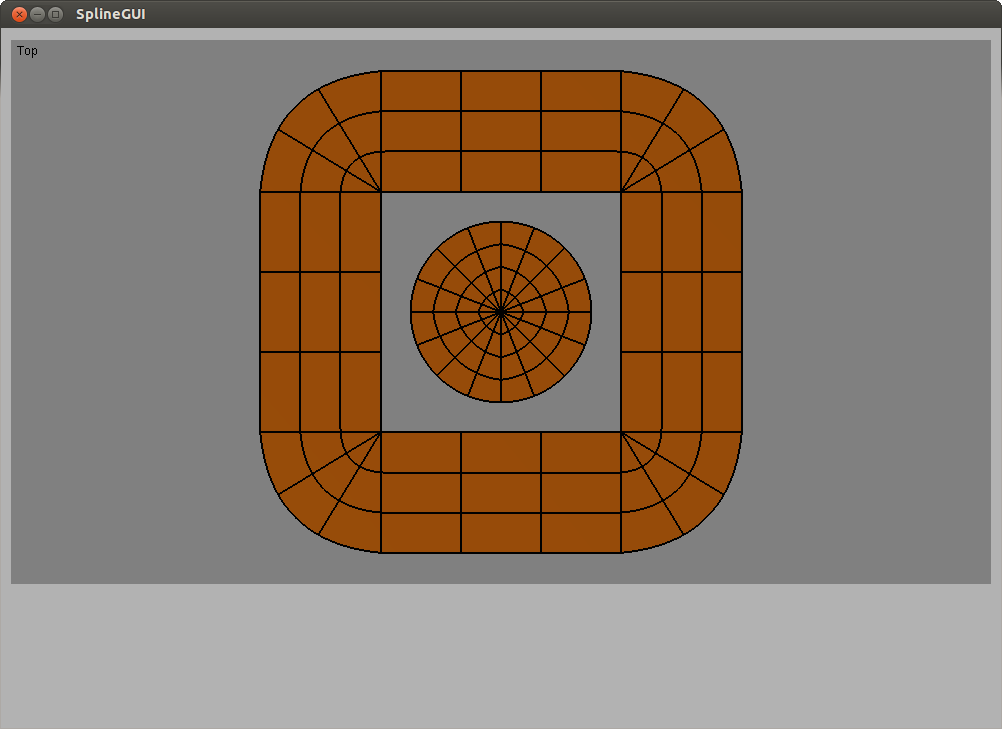
\includegraphics[width=\linewidth]{ntnu5}
    \end{column}
\end{columns}

\end{frame}

%%%%%%%%%%%%%%%%%%%%%%%%%%%%%%%%%%%%%%%%%%%%%%%%%%%%%%%%%%%%%%%%%%%%%%%%%%%%%%%%%%%%%%%%%%%%%%%%%%%%%%%%%%%%%%%%%

\begin{frame}[fragile]
\frametitle{Examples:}
\textbf{Examples:}
\begin{columns}
    \begin{column}{.50\linewidth}
        \begin{listing}[H]
            \tiny
            \begin{minted}{python}
import CurveFactory   as cf
import SurfaceFactory as sf
from math import pi

x  = cf.line([-.5, 0], [.5, 0]) # just to show the origin
y  = cf.line([0, -.5], [0, .5]) # just to show the origin

c1 = cf.circle_segment(pi/2)
c2 = cf.line([0,1], [-4,1])
c1.append(c2)
c1 += (2, 2)
c2 = c1.clone().rotate(pi/2)
c1.append(c2)
c2 = c1.clone().rotate(pi)
c1.append(c2)

s1 = sf.thicken(c1, 1)
s2 = sf.disc(1.5, 'square')
s1.refine(2)
s2.refine(3)

f = open('ntnu.g2', 'w')
s1.write_g2(f)

# x.write_g2(f)
# y.write_g2(f)
            \end{minted}
        \end{listing}
    \end{column}
    \begin{column}{.45\linewidth}
        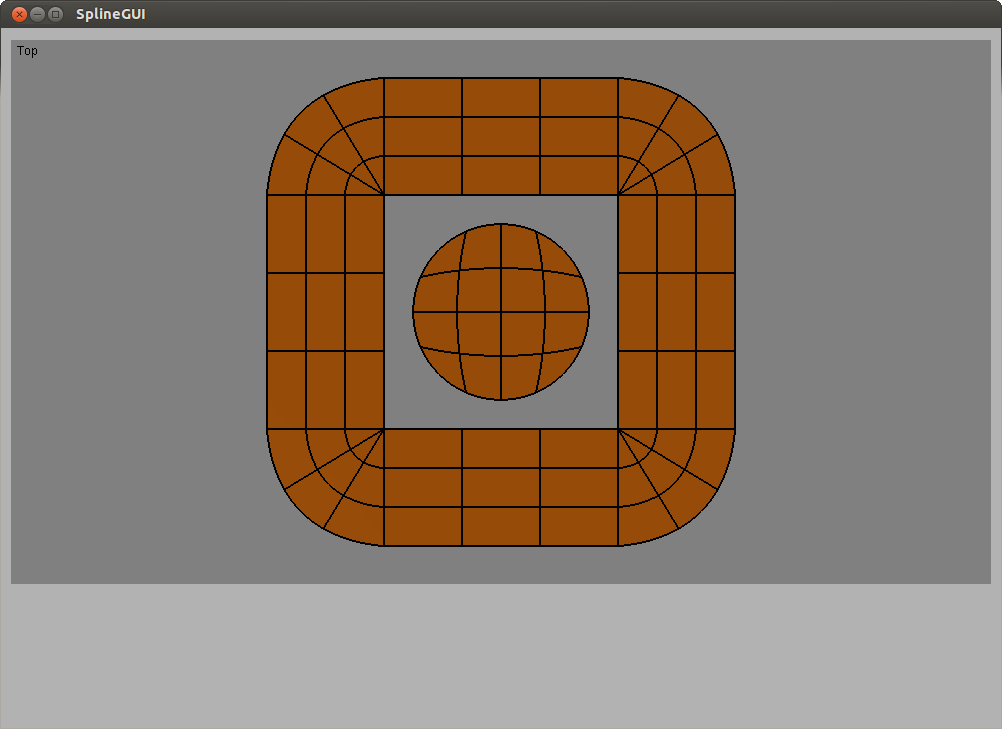
\includegraphics[width=\linewidth]{ntnu6}
    \end{column}
\end{columns}

\end{frame}

%%%%%%%%%%%%%%%%%%%%%%%%%%%%%%%%%%%%%%%%%%%%%%%%%%%%%%%%%%%%%%%%%%%%%%%%%%%%%%%%%%%%%%%%%%%%%%%%%%%%%%%%%%%%%%%%%

\begin{frame}[fragile]
\frametitle{Spline Evaluations:}
\textbf{Spline Evaluations:}
\begin{listing}[H]
    \tiny
    \begin{minted}{python}
import CurveFactory
from math import pi

c = CurveFactory.circle()
c.start()                   # parametric start of domain, here 0
c.end()                     # parametric end   of domain  here 2*pi

c.evaluate(pi/4)            # evaluate (x,y)-coordinate at t=pi/4
c(pi/4)                     # same as above
c(0)                        # evaluate curve at t=0
c[0]                        # return first control point of curve

c.evaluate_tangent(pi/2)    # evaluate tangent vector at t=pi/2
c.evaluate_derivative(pi/2) # same as above

t = [0,.1,.2,.3,.4,.5,.6,.7,.8,.9,1]
x = c(t) # evaluate at all t points, returns matrix x of size 11x2

c(3*pi)  # =c(pi), defined as a periodic spline. Well defined for all t
    \end{minted}
\end{listing}

\end{frame}

%%%%%%%%%%%%%%%%%%%%%%%%%%%%%%%%%%%%%%%%%%%%%%%%%%%%%%%%%%%%%%%%%%%%%%%%%%%%%%%%%%%%%%%%%%%%%%%%%%%%%%%%%%%%%%%%%

\begin{frame}[fragile]
\frametitle{Spline Evaluations:}
\textbf{Spline Evaluations:}
\begin{listing}[H]
    \tiny
    \begin{minted}{python}
from Surface import *
import VolumeFactory
from math import pi

basis = BSplineBasis(3, [0,0,0,1,1,1])
controlpoints = [[0,0], [1,0], [2,0],
                 [0,1], [1,1], [2,1],
                 [0,2], [1,2], [2,2]]
surf = Surface(basis, basis, controlpoints)

surf.start()                   # parametric start of domain, here (0,0)
surf.end()                     # parametric end   of domain  here (1,1)

surf(0.3, 0.4)                 # evaluate surface at (u,v)=(.3,.4)
surf(-0.2, 0.5)                # evaluate outside domain, creates error
surf[0]                        # returns first control-point [0,0]
surf[3]                        # returns 4th control-point [0,1]

u = [0, .2, .4, .6, .8, 1]
v = [0, .2, .4, .6, .8, 1]
x = surf(u,v) # evaluates at all points, returns 3D tensor of size (6,6,2)
x[1,2,0]      # x-coordinate of surface evaluated at (.2, .4)
x[1,2,1]      # y-coordinate of surface evaluated at (.2, .4)

vol = VolumeFactory.extrude(surf,1) # create a volume from the surface
w = [0, .2, .4, .6, .8, 1]
x = vol(u,v,w) # returns a 4D-tensor of size (6,6,6,2)
x[3,4,5,:]     # (x,y) coordinate of volume evaluated at (.6, .8, 1.0)
    \end{minted}
\end{listing}

\end{frame}

%%%%%%%%%%%%%%%%%%%%%%%%%%%%%%%%%%%%%%%%%%%%%%%%%%%%%%%%%%%%%%%%%%%%%%%%%%%%%%%%%%%%%%%%%%%%%%%%%%%%%%%%%%%%%%%%%

\begin{frame}[fragile]
\frametitle{Spline Evaluations:}
\textbf{Spline Evaluations:}

Uses efficient evaluations through numpy tensor products

\begin{listing}[H]
    \tiny
    \begin{minted}{python}
# compute basis functions for all points t. Nu(i,j) is a matrix of all functions j for all points u[i]
Nu = self.basis1.evaluate(u)
Nv = self.basis2.evaluate(v)
Nw = self.basis3.evaluate(w)

# compute physical points [x,y,z] for all points (u[i],v[j],w[k]). For rational volumes, compute [X,Y,Z,W] (in projective space)
result = np.tensordot(Nw, self.controlpoints, axes=(1,2))
result = np.tensordot(Nv, result,             axes=(1,2))
result = np.tensordot(Nu, result,             axes=(1,2))

# Project rational volumes down to geometry space: x = X/W, y=Y/W, z=Z/W
if self.rational: 
    for i in range(self.dimension):
        result[:,:,:,i] /= result[:,:,:,-1] 
    \end{minted}
\end{listing}

\end{frame}

%%%%%%%%%%%%%%%%%%%%%%%%%%%%%%%%%%%%%%%%%%%%%%%%%%%%%%%%%%%%%%%%%%%%%%%%%%%%%%%%%%%%%%%%%%%%%%%%%%%%%%%%%%%%%%%%%

\begin{frame}[fragile]
\frametitle{Spline Interpolation:}
\textbf{Spline Interpolation:}

Uses efficient evaluations through numpy tensor products

\begin{listing}[H]
    \tiny
    \begin{minted}{python}
# compute interpolations points
u = self.basis1.greville()
v = self.basis2.greville()
w = self.basis3.greville()

# compute basis function matrices
Nu = self.basis1.evaluate( u )
Nv = self.basis2.evaluate( v )
Nw = self.basis3.evaluate( w )

# solve the interpolation problem
Nu_inv = np.linalg.inv(Nu)
Nv_inv = np.linalg.inv(Nv)
Nw_inv = np.linalg.inv(Nw) # these are inverses of the 1D problems, and small compared to the total number of unknowns
tmp = np.tensordot(Nw_inv, interpolation_pts_x, axes=(1,2))
tmp = np.tensordot(Nv_inv, tmp,                 axes=(1,2))
tmp = np.tensordot(Nu_inv, tmp,                 axes=(1,2))

self.controlpoints = tmp
    \end{minted}
\end{listing}

\end{frame}

%%%%%%%%%%%%%%%%%%%%%%%%%%%%%%%%%%%%%%%%%%%%%%%%%%%%%%%%%%%%%%%%%%%%%%%%%%%%%%%%%%%%%%%%%%%%%%%%%%%%%%%%%%%%%%%%%

\begin{frame}[fragile]
\frametitle{Affine transformation}
\textbf{Affine transformation:}

Standard 4x4 matrices for move,rotate,etc

\begin{listing}[H]
    \tiny
    \begin{minted}{python}
def translate(self, x):
# 3D rational example: create a 4x4 translation matrix
#
#  |xw|      |  1   0   0  x1 |   |xw|
#  |yw|   =  |  0   1   0  x2 | * |yw|
#  |zw|      |  0   0   1  x3 |   |zw|
#  | w|_new  |  0   0   0   1 |   | w|_old
# 
dim = self.dimension
rat = self.rational
n   = len(self)  # number of control points

# set up the translation matrix
translation_matrix = np.matrix(np.identity(dim+1))
for i in range(dim):
    translation_matrix[i,-1] = x[i]

# wrap out the controlpoints to a matrix (down from n-D tensor)
cp = np.matrix(np.reshape(self.controlpoints, (n, dim+rat)))

# do the actual scaling by matrix-matrix multiplication
cp  = cp * translation_matrix.T # right-mult, so we need transpose

# store results
self.controlpoints = np.reshape(np.array(cp), self.controlpoints.shape)

return self
    \end{minted}
\end{listing}

\end{frame}

%%%%%%%%%%%%%%%%%%%%%%%%%%%%%%%%%%%%%%%%%%%%%%%%%%%%%%%%%%%%%%%%%%%%%%%%%%%%%%%%%%%%%%%%%%%%%%%%%%%%%%%%%%%%%%%%%

\begin{frame}[fragile]
\frametitle{Flow around a cylinder}
\textbf{Flow around a cylinder}

\begin{columns}
    \begin{column}{.50\linewidth}
        \begin{listing}[H]
            \tiny
            \begin{minted}{python}
from math import pi
import CurveFactory   as cf
import SurfaceFactory as sf


circle    = cf.circle(1.0)
boundary  = cf.n_gon(4)
boundary *= 4




f = open('flow-around-cylinder.g2', 'w')
circle.write_g2(f)
boundary.write_g2(f)
            \end{minted}
        \end{listing}
    \end{column}
    \begin{column}{.45\linewidth}
        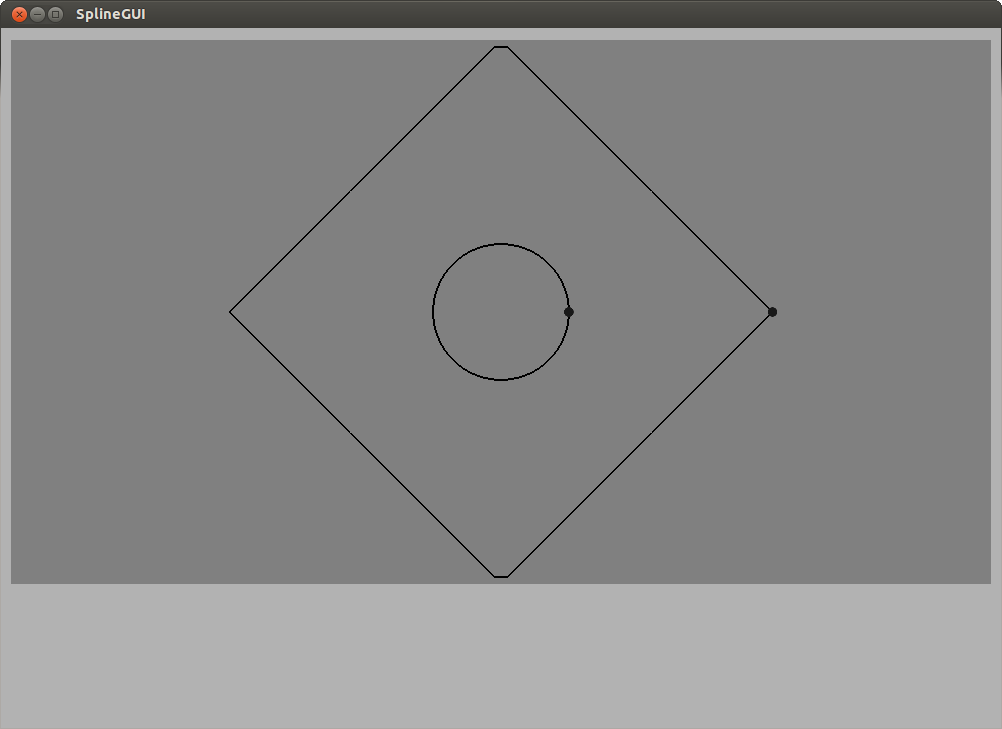
\includegraphics[width=\linewidth]{cylinder1}
    \end{column}
\end{columns}

\end{frame}

%%%%%%%%%%%%%%%%%%%%%%%%%%%%%%%%%%%%%%%%%%%%%%%%%%%%%%%%%%%%%%%%%%%%%%%%%%%%%%%%%%%%%%%%%%%%%%%%%%%%%%%%%%%%%%%%%

\begin{frame}[fragile]
\frametitle{Flow around a cylinder}
\textbf{Flow around a cylinder}

\begin{columns}
    \begin{column}{.50\linewidth}
        \begin{listing}[H]
            \tiny
            \begin{minted}{python}
from math import pi
import CurveFactory   as cf
import SurfaceFactory as sf


circle    = cf.circle(1.0)
boundary  = cf.n_gon(4)
boundary *= 4
surf      = sf.edge_curves([circle, boundary])

surf.rotate(pi/4)

f = open('flow-around-cylinder.g2', 'w')

surf.write_g2(f)
            \end{minted}
        \end{listing}
    \end{column}
    \begin{column}{.45\linewidth}
        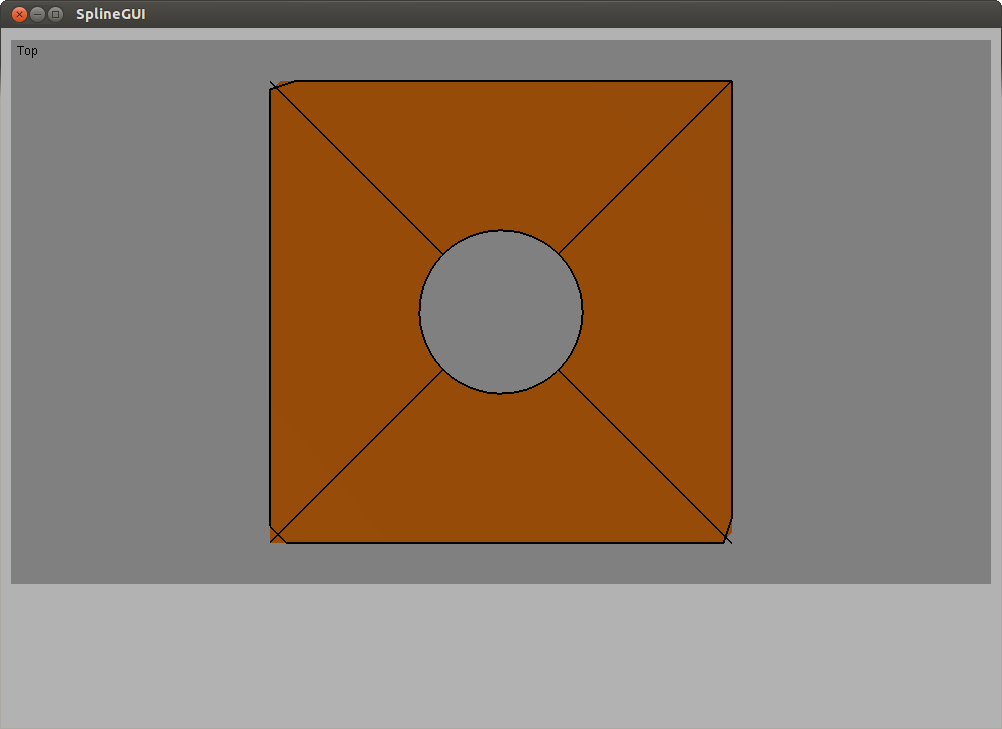
\includegraphics[width=\linewidth]{cylinder2}
    \end{column}
\end{columns}

\end{frame}

%%%%%%%%%%%%%%%%%%%%%%%%%%%%%%%%%%%%%%%%%%%%%%%%%%%%%%%%%%%%%%%%%%%%%%%%%%%%%%%%%%%%%%%%%%%%%%%%%%%%%%%%%%%%%%%%%

\begin{frame}[fragile]
\frametitle{Building a nut}
\textbf{Building a nut}

\begin{columns}
    \begin{column}{.50\linewidth}
        \begin{listing}[H]
            \tiny
            \begin{minted}{python}
from math import pi
import CurveFactory   as cf
import SurfaceFactory as sf


circle    = cf.circle(1.0)
boundary  = cf.n_gon(6)
boundary *= 2.4




f = open('nut.g2', 'w')
circle.write_g2(f)
boundary.write_g2(f)
            \end{minted}
        \end{listing}
    \end{column}
    \begin{column}{.45\linewidth}
        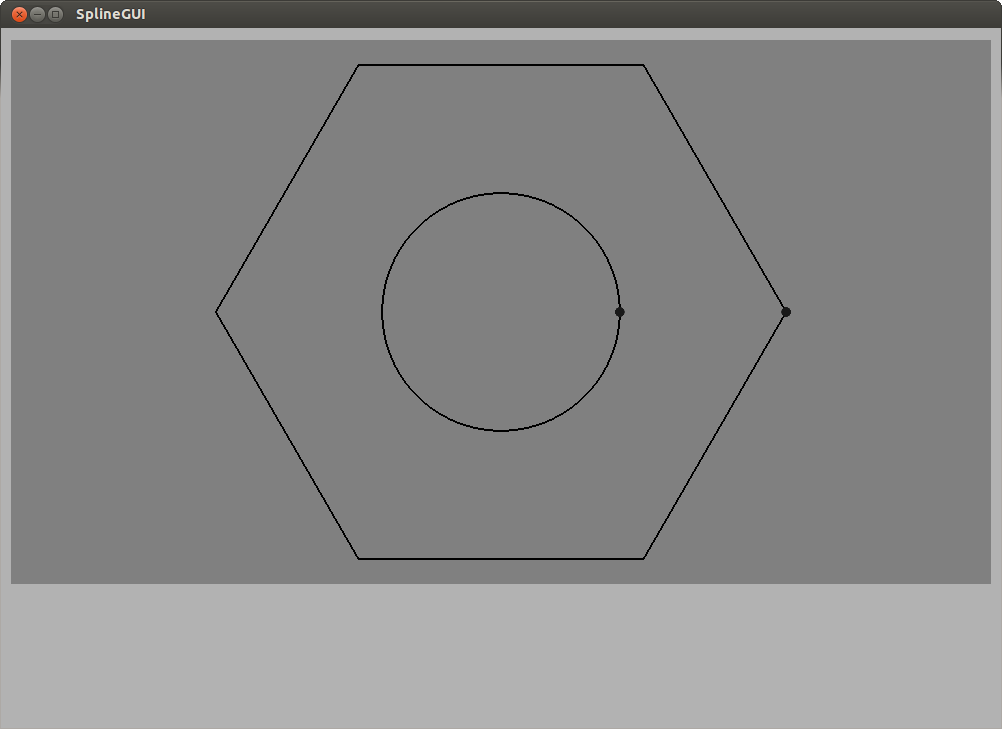
\includegraphics[width=\linewidth]{nut1}
    \end{column}
\end{columns}

\end{frame}

%%%%%%%%%%%%%%%%%%%%%%%%%%%%%%%%%%%%%%%%%%%%%%%%%%%%%%%%%%%%%%%%%%%%%%%%%%%%%%%%%%%%%%%%%%%%%%%%%%%%%%%%%%%%%%%%%

\begin{frame}[fragile]
\frametitle{Building a nut}
\textbf{Building a nut}

\begin{columns}
    \begin{column}{.50\linewidth}
        \begin{listing}[H]
            \tiny
            \begin{minted}{python}
from math import pi
import CurveFactory   as cf
import SurfaceFactory as sf
import VolumeFactory  as vf

circle    = cf.circle(1.0)
boundary  = cf.n_gon(6)
boundary *= 2.4
surf      = sf.edge_curves([circle, boundary])

vol       = vf.extrude(surf, 2)

f = open('nut.g2', 'w')

vol.write_g2(f)
            \end{minted}
        \end{listing}
    \end{column}
    \begin{column}{.45\linewidth}
        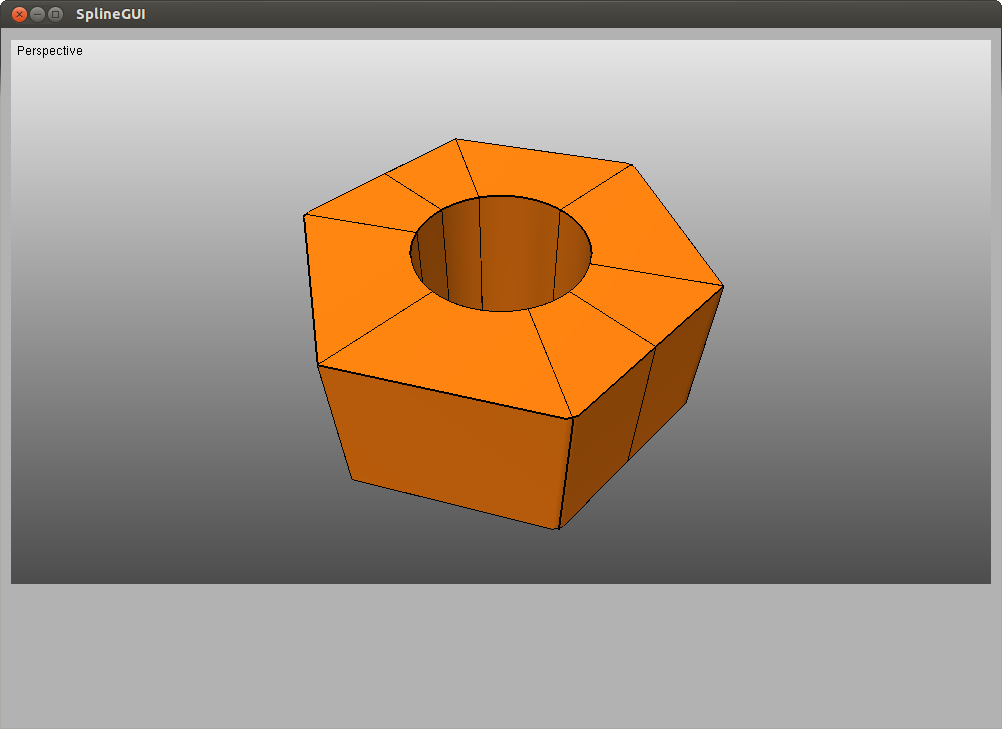
\includegraphics[width=\linewidth]{nut2}
    \end{column}
\end{columns}

\end{frame}

%%%%%%%%%%%%%%%%%%%%%%%%%%%%%%%%%%%%%%%%%%%%%%%%%%%%%%%%%%%%%%%%%%%%%%%%%%%%%%%%%%%%%%%%%%%%%%%%%%%%%%%%%%%%%%%%%

\begin{frame}[fragile]
\frametitle{NACA wing profile}
\textbf{NACA wing profile}

\begin{figure}[h]
    \centering
    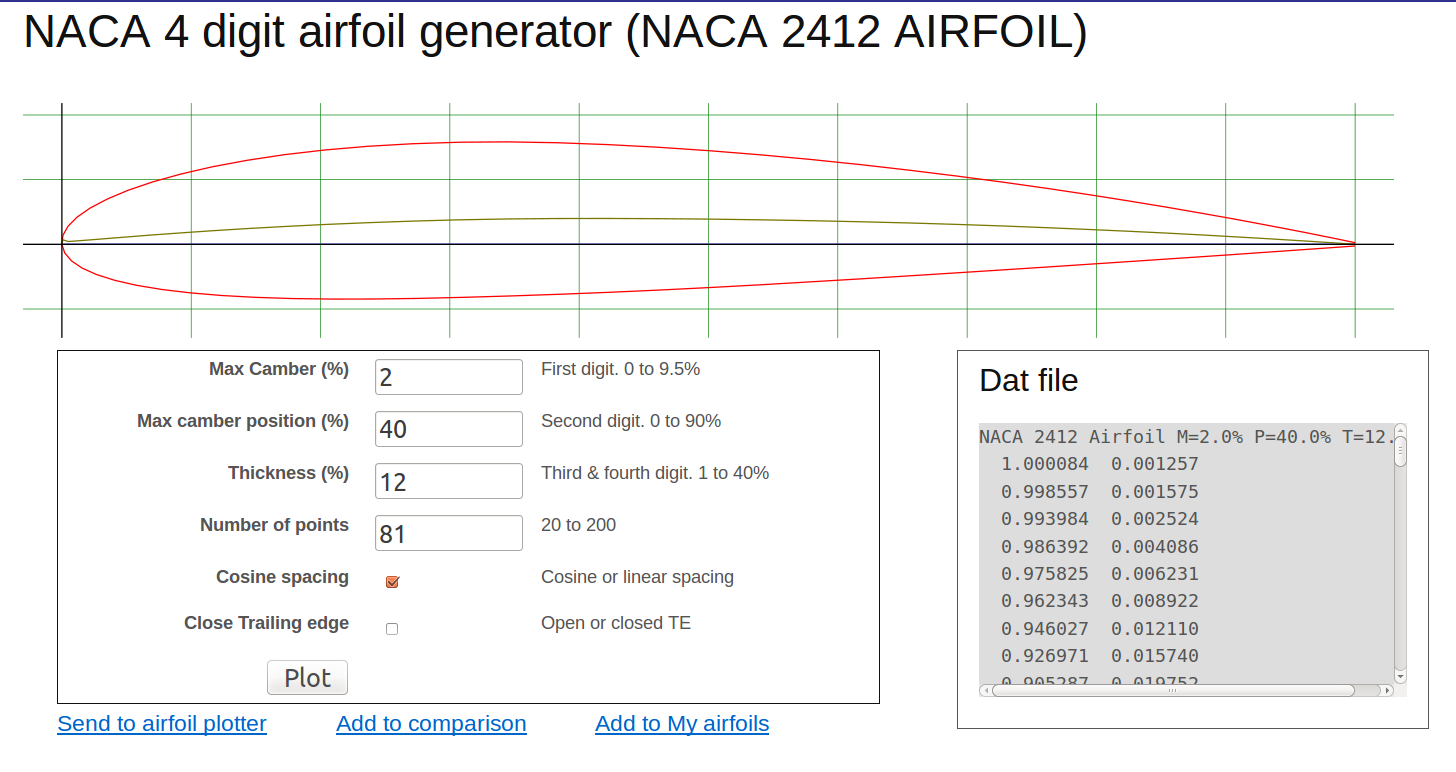
\includegraphics[width=0.8\linewidth]{naca-webpage}
\end{figure}
%\vspace{2cm}
\url{http://airfoiltools.com/airfoil/naca4digit}

\end{frame}

%%%%%%%%%%%%%%%%%%%%%%%%%%%%%%%%%%%%%%%%%%%%%%%%%%%%%%%%%%%%%%%%%%%%%%%%%%%%%%%%%%%%%%%%%%%%%%%%%%%%%%%%%%%%%%%%%

\begin{frame}[fragile]
\frametitle{NACA wing profile}
\textbf{NACA wing profile}

Center line (camber)
\begin{equation*}
    y(x) = \left\{
    \begin{array}{ll}
        \frac{M}{P^2}(2Px-x^2)          & 0\leq x\leq P \\
        \frac{M}{(1-P)^2}(1-2P+2Px-x^2) & P\leq x\leq 1 \\
    \end{array}
    \right.
\end{equation*}
\begin{listing}[H]
    \tiny
    \begin{minted}{python}
from Curve import *
import CurveFactory
import numpy as np

def camber(M,P):
    basis = BSplineBasis(3) # quadratic basis
    basis.insert_knot(P)    # create C1-knot at P

    t = basis.greville()    # interpolation points
    n = len(t)              # number of basis functions (=4)
    x = np.zeros((n,2))
    for i in range(n):
        if t[i] <= P:
            x[i,0] = t[i]
            x[i,1] = M/P/P*(2*P*t[i] - t[i]*t[i])
        else:
            x[i,0] = t[i]
            x[i,1] = M/(1-P)/(1-P)*(1-2*P + 2*P*t[i] - t[i]*t[i])

    return CurveFactory.interpolate(x, basis)
    \end{minted}
\end{listing}

\end{frame}

%%%%%%%%%%%%%%%%%%%%%%%%%%%%%%%%%%%%%%%%%%%%%%%%%%%%%%%%%%%%%%%%%%%%%%%%%%%%%%%%%%%%%%%%%%%%%%%%%%%%%%%%%%%%%%%%%

\begin{frame}
\frametitle{NACA wing profile}
\textbf{NACA wing profile}

Previous parametrization used
\begin{eqnarray*}
    x(t) & = & t \\
    y(t) & = & \left\{
    \begin{array}{ll}
        \frac{M}{P^2}(2Px-t^2)          & 0\leq t\leq P \\
        \frac{M}{(1-P)^2}(1-2P+2Px-t^2) & P\leq t\leq 1 \\
    \end{array} \right.
\end{eqnarray*}
\pause
but it is well known that $x(t)=t$ is a suboptimal parametrization.
Webpage suggests
\begin{equation*}
    x(t) = \frac{1}{2}\left(1-cos(t)\right), 0\leq t\leq \pi
\end{equation*}
\pause
but might as well choose a piecewise polynomial
\begin{equation*}
    x(t) = \left\{
        \begin{array}{ll}
             2t^2                  & 0 \leq t \leq \frac{1}{2} \\
            -2(t^2-2t+\frac{1}{2}) & \frac{1}{2} \leq t \leq 1
        \end{array}
    \right.
\end{equation*}

\end{frame}

%%%%%%%%%%%%%%%%%%%%%%%%%%%%%%%%%%%%%%%%%%%%%%%%%%%%%%%%%%%%%%%%%%%%%%%%%%%%%%%%%%%%%%%%%%%%%%%%%%%%%%%%%%%%%%%%%

\begin{frame}
\frametitle{NACA wing profile}
\textbf{NACA wing profile}

\begin{figure}[h]
    \centering
    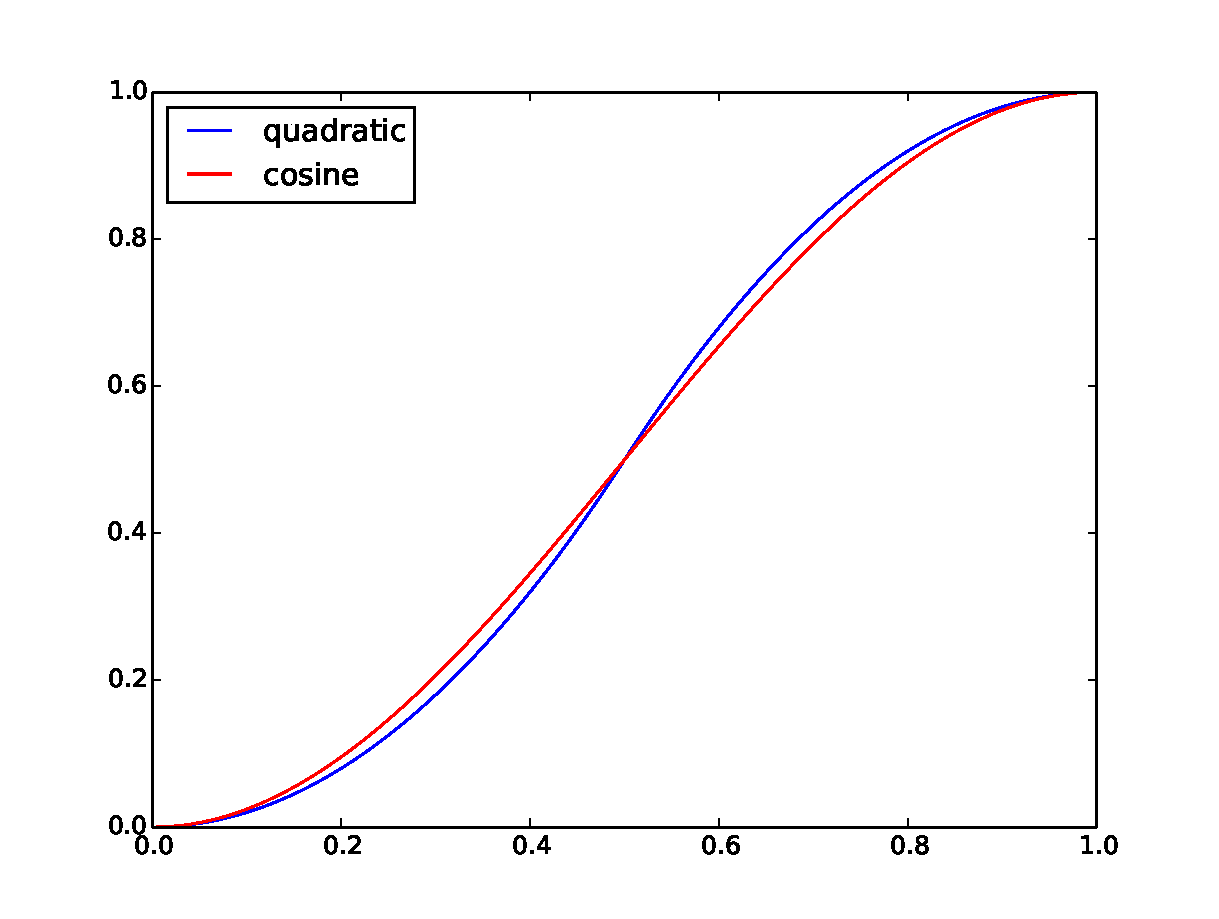
\includegraphics[width=0.5\linewidth]{parametrization}
\end{figure}

\begin{equation*}
    x(t) = \frac{1}{2}\left(1-cos(t)\right), 0\leq t\leq \pi
\end{equation*}
\begin{equation*}
    x(t) = \left\{
        \begin{array}{ll}
             2t^2                  & 0 \leq t \leq \frac{1}{2} \\
            -2(t^2-2t+\frac{1}{2}) & \frac{1}{2} \leq t \leq 1
        \end{array}
    \right.
\end{equation*}

\end{frame}

%%%%%%%%%%%%%%%%%%%%%%%%%%%%%%%%%%%%%%%%%%%%%%%%%%%%%%%%%%%%%%%%%%%%%%%%%%%%%%%%%%%%%%%%%%%%%%%%%%%%%%%%%%%%%%%%%

\begin{frame}[fragile]
\frametitle{NACA wing profile}
\textbf{NACA wing profile}

\begin{listing}[H]
    \tiny
    \begin{minted}{python}
from Curve import *
import CurveFactory
import numpy as np

def camber(M,P):
    basis = BSplineBasis(5)       # p=4 basis
    basis.insert_knot([P,P,P])    # create C1-knot at P for y-parametrization
    basis.insert_knot([.5,.5,.5]) # create C1-knot at 0.5 for x-parametrization

    t = basis.greville()    # interpolation points
    n = len(t)              # number of basis functions
    x = np.zeros((n,2))
    for i in range(n):
        if t[i] <= 0.5:
            x[i,0] = t[i]**2 / P
        else:
            x[i,0] = -2*(t[i]**2-2*t[i]+.5)
        if t[i] <= P:
            x[i,1] = M/P/P*(2*P*x[i,0] - x[i,0]*x[i,0])
        else:
            x[i,1] = M/(1-P)/(1-P)*(1-2*P + 2*P*x[i,0] - x[i,0]*x[i,0])

    return CurveFactory.interpolate(x, basis)
    \end{minted}
\end{listing}

\end{frame}

%%%%%%%%%%%%%%%%%%%%%%%%%%%%%%%%%%%%%%%%%%%%%%%%%%%%%%%%%%%%%%%%%%%%%%%%%%%%%%%%%%%%%%%%%%%%%%%%%%%%%%%%%%%%%%%%%

\begin{frame}[fragile]
\frametitle{NACA wing profile}
\textbf{NACA wing profile}

\begin{columns}
    \begin{column}{.50\linewidth}
        \begin{listing}[H]
            \tiny
            \begin{minted}{python}
from SurfaceFactory import *
from math import *

c = camber(2,4)








    
c.insert_knot([.1, .2, .3, .6, .7, .8, .9])
s = thicken(c, .05)

f = open('naca.g2', 'w')
s.write_g2(f)
c.write_g2(f)

            \end{minted}
        \end{listing}
    \end{column}
    \begin{column}{.45\linewidth}
        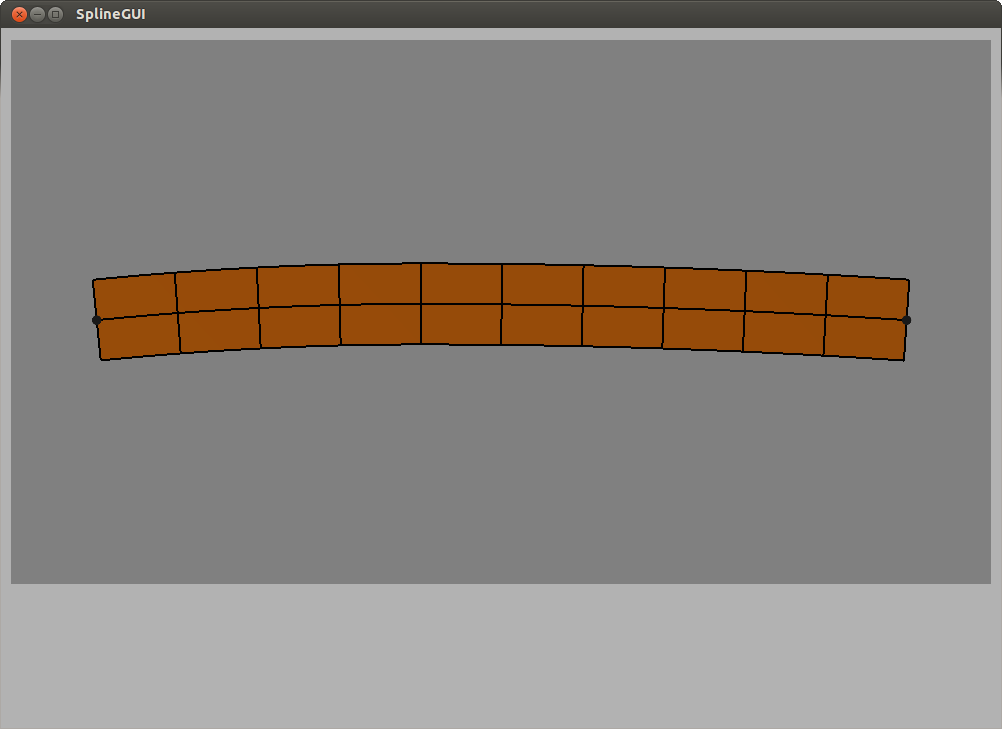
\includegraphics[width=\linewidth]{naca1}
    \end{column}
\end{columns}
\end{frame}

%%%%%%%%%%%%%%%%%%%%%%%%%%%%%%%%%%%%%%%%%%%%%%%%%%%%%%%%%%%%%%%%%%%%%%%%%%%%%%%%%%%%%%%%%%%%%%%%%%%%%%%%%%%%%%%%%

\begin{frame}[fragile]
\frametitle{NACA wing profile}
\textbf{NACA wing profile}

\begin{columns}
    \begin{column}{.50\linewidth}
        \begin{listing}[H]
            \tiny
            \begin{minted}{python}
from SurfaceFactory import *
from math import *

c = camber(2,4)
def thickness(x):
    T  = 0.12
    a0 = 0.2969
    a1 = -0.126
    a2 = -0.3516
    a3 = 0.2843
    a4 = -0.1015
    return T/0.2*(a0*sqrt(x) + a1*x + a2*x**2 + a3*x**3 + a4*x**4)
    
c.insert_knot([.1, .2, .3, .6, .7, .8, .9])
s = thicken(c, thickness)

f = open('naca.g2', 'w')
s.write_g2(f)
c.write_g2(f)

            \end{minted}
        \end{listing}
    \end{column}
    \begin{column}{.45\linewidth}
        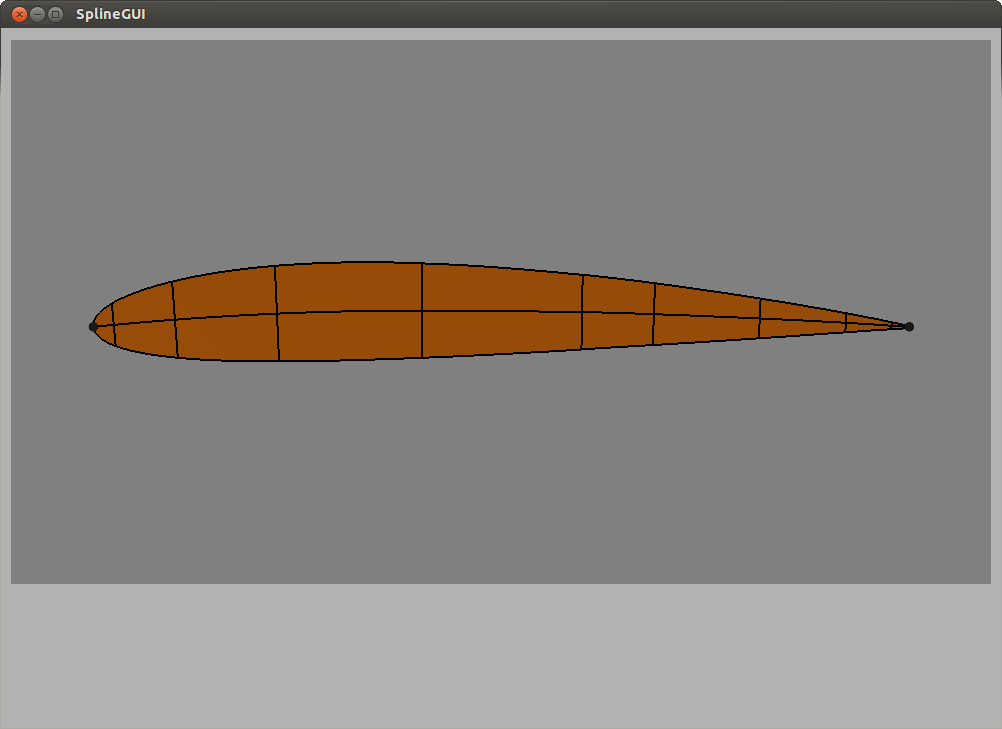
\includegraphics[width=\linewidth]{naca2}
    \end{column}
\end{columns}
\end{frame}

%%%%%%%%%%%%%%%%%%%%%%%%%%%%%%%%%%%%%%%%%%%%%%%%%%%%%%%%%%%%%%%%%%%%%%%%%%%%%%%%%%%%%%%%%%%%%%%%%%%%%%%%%%%%%%%%%

\begin{frame}[fragile]
\frametitle{NACA wing profile}
\textbf{NACA wing profile}

\begin{columns}
    \begin{column}{.50\linewidth}
        \begin{listing}[H]
            \tiny
            \begin{minted}{python}
from SurfaceFactory import *
from math import *

c = camber(2,4)
def thickness(t):
    T  = 0.12
    a0 = 0.2969
    a1 = -0.126
    a2 = -0.3516
    a3 = 0.2843
    a4 = -0.1015
    return T/0.2*(a0*sqrt(t) + a1*t + a2*t**2 + a3*t**3 + a4*t**4)
    
c.insert_knot([.1, .2, .3, .6, .7, .8, .9])
s = thicken(c, thickness)

f = open('naca.g2', 'w')
s.write_g2(f)
c.write_g2(f)

            \end{minted}
        \end{listing}
    \end{column}
    \begin{column}{.45\linewidth}
        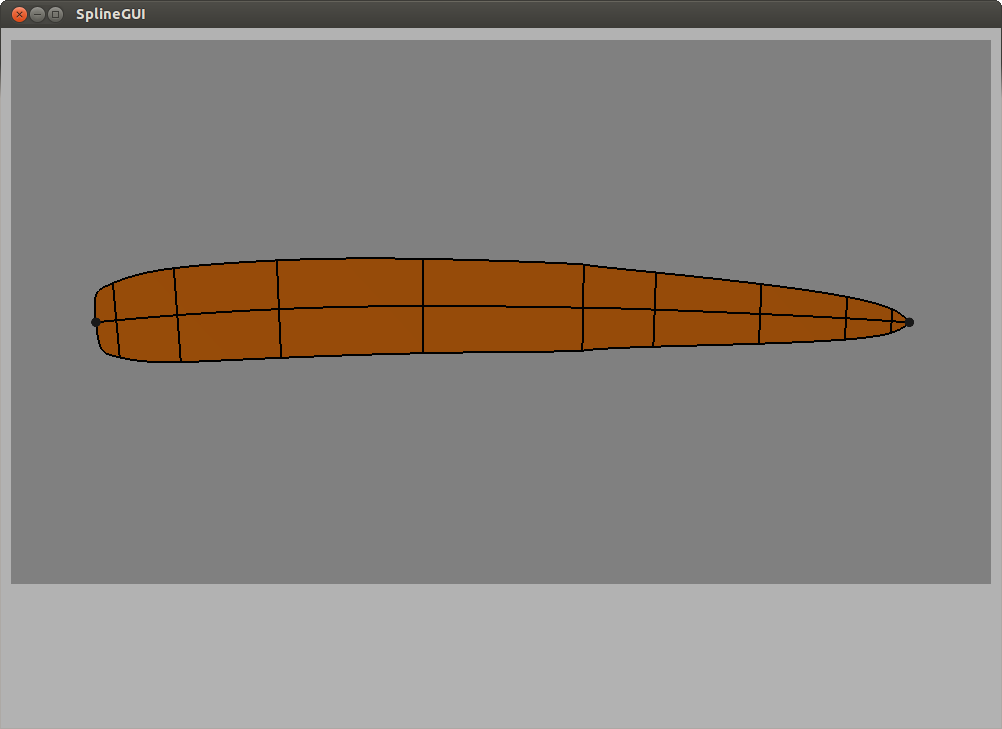
\includegraphics[width=\linewidth]{naca3}
    \end{column}
\end{columns}
\end{frame}

%%%%%%%%%%%%%%%%%%%%%%%%%%%%%%%%%%%%%%%%%%%%%%%%%%%%%%%%%%%%%%%%%%%%%%%%%%%%%%%%%%%%%%%%%%%%%%%%%%%%%%%%%%%%%%%%%

\begin{frame}[fragile]
\frametitle{NACA wing profile}
\textbf{NACA wing profile}

\begin{columns}
    \begin{column}{.50\linewidth}
        \begin{listing}[H]
            \tiny
            \begin{minted}{python}
from SurfaceFactory import *
from math import *

c = camber(2,4)
def thickness(y):
    T  = 0.12
    a0 = 0.2969
    a1 = -0.126
    a2 = -0.3516
    a3 = 0.2843
    a4 = -0.1015
    return T/0.2*(a0*sqrt(y) + a1*y + a2*y**2 + a3*y**3 + a4*y**4)
    
c.insert_knot([.1, .2, .3, .6, .7, .8, .9])
s = thicken(c, thickness)

f = open('naca.g2', 'w')
s.write_g2(f)
c.write_g2(f)

            \end{minted}
        \end{listing}
    \end{column}
    \begin{column}{.45\linewidth}
        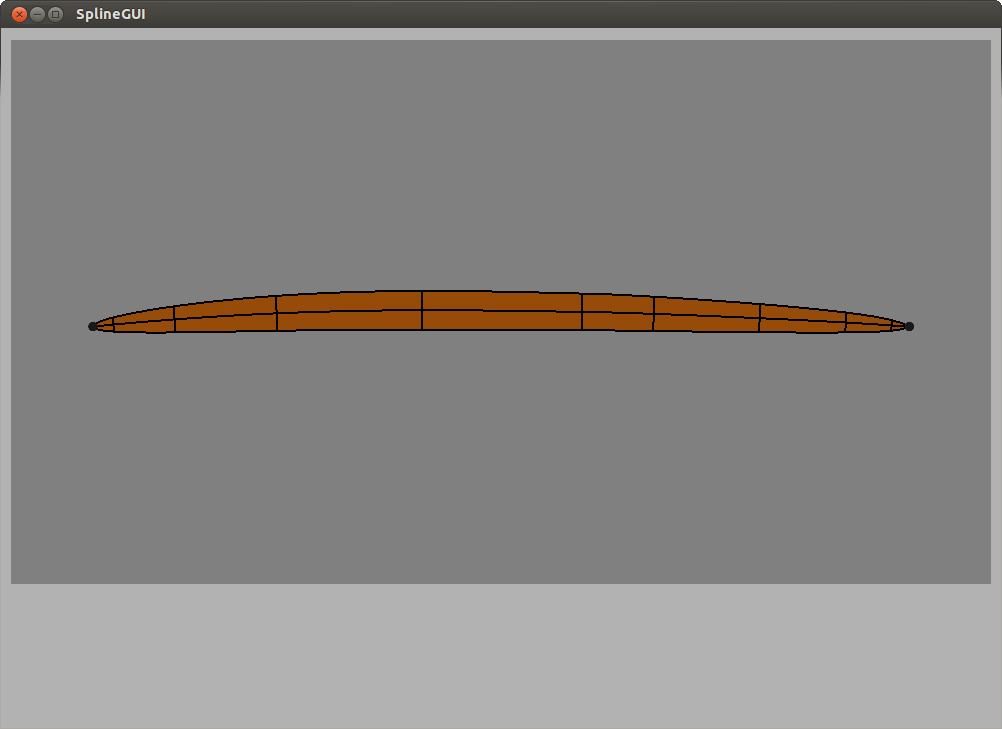
\includegraphics[width=\linewidth]{naca4}
    \end{column}
\end{columns}
\end{frame}

%%%%%%%%%%%%%%%%%%%%%%%%%%%%%%%%%%%%%%%%%%%%%%%%%%%%%%%%%%%%%%%%%%%%%%%%%%%%%%%%%%%%%%%%%%%%%%%%%%%%%%%%%%%%%%%%%

\begin{frame}[fragile]
\frametitle{NACA wing profile}
\textbf{NACA wing profile}

\begin{columns}
    \begin{column}{.50\linewidth}
        \begin{listing}[H]
            \tiny
            \begin{minted}{python}
from SurfaceFactory import *
from math import *

c = camber(2,4)
def thickness(t):
    return t*(1-t)*(sin(4*pi*t)+1.5)






    
c.insert_knot([.1, .2, .3, .6, .7, .8, .9])
s = thicken(c, thickness)

f = open('naca.g2', 'w')
s.write_g2(f)
c.write_g2(f)

            \end{minted}
        \end{listing}
    \end{column}
    \begin{column}{.45\linewidth}
        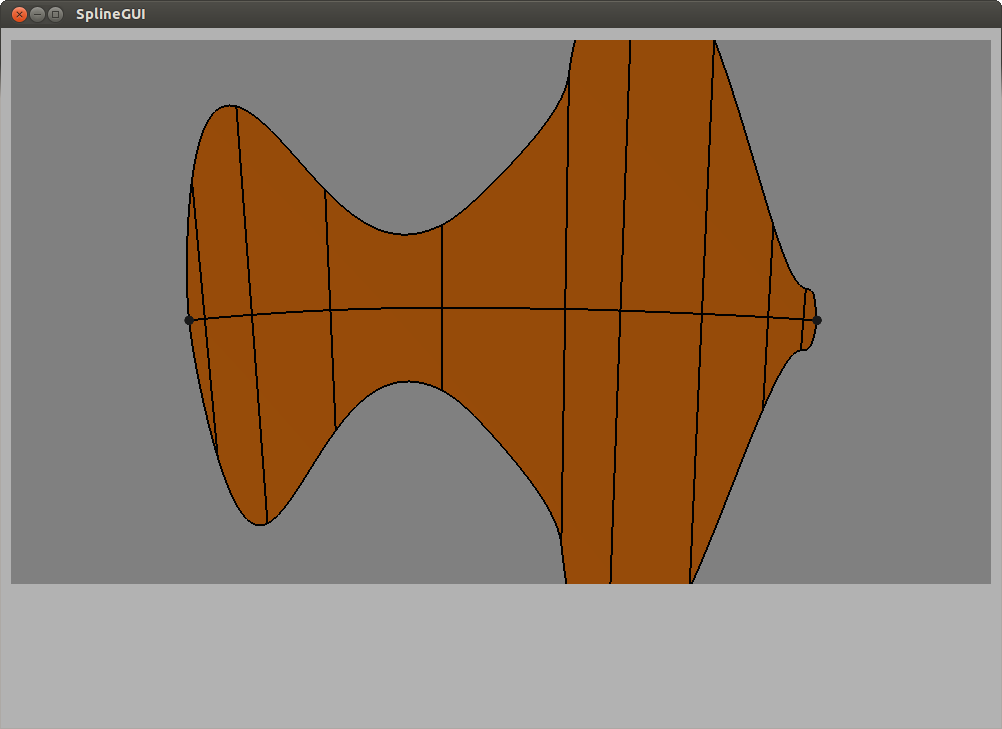
\includegraphics[width=\linewidth]{naca5}
    \end{column}
\end{columns}

\end{frame}

%%%%%%%%%%%%%%%%%%%%%%%%%%%%%%%%%%%%%%%%%%%%%%%%%%%%%%%%%%%%%%%%%%%%%%%%%%%%%%%%%%%%%%%%%%%%%%%%%%%%%%%%%%%%%%%%%

\begin{frame}
\frametitle{What it doesn't do}
\textbf{What it doesn't do}
\begin{itemize}
    \item No point \& click user interface
    \item No automatic topology solutions for multi-patch problems
    \item No boolean operations (union $A\bigcup B$ or intersection $A\bigcap B$)
    \item No trimming
\end{itemize}
\end{frame}

%%%%%%%%%%%%%%%%%%%%%%%%%%%%%%%%%%%%%%%%%%%%%%%%%%%%%%%%%%%%%%%%%%%%%%%%%%%%%%%%%%%%%%%%%%%%%%%%%%%%%%%%%%%%%%%%%

\begin{frame}
\frametitle{What it does}
\textbf{What it does}
\begin{itemize}
    \item Spline evaluations (and derivatives, tangents, normals)
    \pause
    \item Elementary operations (move, scale, rotate, etc)
    \pause
    \item Spline operations (extrude, loft, revolve, sweep)
    \pause
    \item Volumetric meshing
    \pause
    \item Interpolations and approximations
\end{itemize}
\pause
\vspace{1cm}
and all of the above works for
\begin{itemize}
    \item Rational splines
    \item Periodic splines
    \item 2D splines
\end{itemize}
\end{frame}

%%%%%%%%%%%%%%%%%%%%%%%%%%%%%%%%%%%%%%%%%%%%%%%%%%%%%%%%%%%%%%%%%%%%%%%%%%%%%%%%%%%%%%%%%%%%%%%%%%%%%%%%%%%%%%%%%

\begin{frame}
\frametitle{Design choices}
\textbf{Design choices}
\begin{itemize}
    \item Stable!
    \begin{itemize}
        \item lots of testing
        \item state assumptions where used
    \end{itemize}
    \pause
    \item Readable
    \begin{itemize}
        \item lots of documentation
        \item lots of code comments
    \end{itemize}
    \pause
    \item Don't have to be perfect
    \begin{itemize}
        \item make it working first
        \item optimize \emph{if needed}
        \pause
        \item \textbf{working} trumphs \textbf{optimized}
    \end{itemize}
    \pause
    \item Easy to learn...
    \begin{itemize}
        \item Simple interface to create simple geometries
    \end{itemize}
    \pause
    \item ...hard to master
    \begin{itemize}
        \item Visibility and control to create complex geometries
    \end{itemize}
\end{itemize}
\end{frame}

%%%%%%%%%%%%%%%%%%%%%%%%%%%%%%%%%%%%%%%%%%%%%%%%%%%%%%%%%%%%%%%%%%%%%%%%%%%%%%%%%%%%%%%%%%%%%%%%%%%%%%%%%%%%%%%%%


\end{document}
